\chapter{三角函数的图象和性质}
我们知道,函数图象能把函数性质形象地表现出来,为了便于研究三角函数的性质,我们现在来做出各三角函数的图象。
\section{正弦函数的图象和性质}
\subsection{正弦函数的图象}

我们知道正弦函数的定义域是$(-\infty, +\infty)$, 且它是个奇函数,故它的图象可在$x$轴的正、负方向无限延伸,且图象关于原点对称。

我们先用描点法作出它的图象,列出$x$由0到$2\pi$每隔$\frac{\pi}{6}$
取值的正弦值表如下:

\begin{center}
\begin{tabular}{c|ccccccc}
    \hline
$x$ & 0& $\frac{\pi}{6}$& $\frac{\pi}{3}$& $\frac{\pi}{2}$& $\frac{2\pi}{3}$& $\frac{5\pi}{6}$& $\pi$\\
$\sin x$ & 0  & $\frac{1}{2}$  & $\frac{\sqrt{3}}{2}$  & 1  & $\frac{\sqrt{3}}{2}$  & $\frac{1}{2}$ & 0\\
\hline
$x$ && $\frac{7\pi}{6}$& $\frac{4\pi}{3}$& $\frac{3\pi}{2}$& $\frac{5\pi}{3}$& $\frac{11\pi}{6}$&$2\pi$\\
$\sin x$ && $-\frac{1}{2}$  & $-\frac{\sqrt{3}}{2}$  & $-1$  & $-\frac{\sqrt{3}}{2}$  & $-\frac{1}{2}$  & 0\\
\hline
\end{tabular}
\end{center}

把表内$x,y$的每一对值作为点的坐标,在直角坐标系内作出对应的点,将它们依次连结成平滑曲线,这条曲线就是$[0, 2\pi]$上正弦函数$y=\sin x$的图象(图7.1)。

\begin{figure}[htp]
    \centering
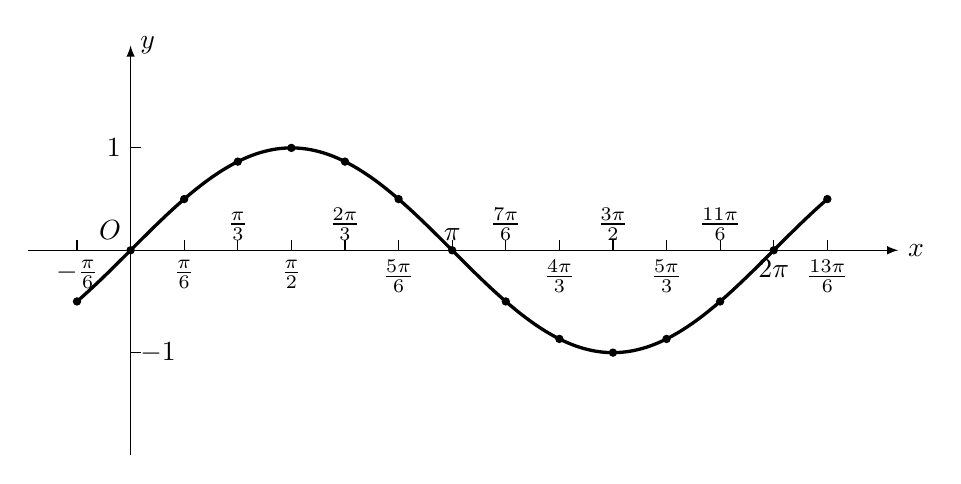
\begin{tikzpicture}[>=latex, scale=1.3]
\draw[->](-1,0)--(7.5,0)node[right]{$x$}; 
\draw [->](0,-2)--(0,2)node[right]{$y$};
    
\draw[domain=-pi/6 :13*pi/6,  samples=1000, very thick] plot(\x, {sin(\x r)});
\foreach \x in {-1,...,13}
{
    \draw (\x/6*pi,0)--(\x/6*pi,.1);
    \draw  (\x/6*pi, {sin(\x/6*pi r)})[fill=black] circle(1pt);
}
\draw (0,1)--(.1,1);
\draw (0,-1)--(.1,-1);
\node at (0,1)[left]{1};
\node at (0,-1)[right]{$-1$};


\node at (-.2,.2){$O$};
\node at (-1/6*pi,0)[below]{$-\frac{\pi}{6}$};
\node at (1/6*pi,0)[below]{$\frac{\pi}{6}$};
\node at (2/6*pi,0)[above]{$\frac{\pi}{3}$};
\node at (3/6*pi,0)[below]{$\frac{\pi}{2}$};
\node at (4/6*pi,0)[above]{$\frac{2\pi}{3}$};
\node at (5/6*pi,0)[below]{$\frac{5\pi}{6}$};
\node at (6/6*pi,0)[above]{$\pi$};
\node at (7/6*pi,0)[above]{$\frac{7\pi}{6}$};
\node at (8/6*pi,0)[below]{$\frac{4\pi}{3}$};
\node at (9/6*pi,0)[above]{$\frac{3\pi}{2}$};
\node at (10/6*pi,0)[below]{$\frac{5\pi}{3}$};
\node at (11/6*pi,0)[above]{$\frac{11\pi}{6}$};
\node at (12/6*pi,0)[below]{$2\pi$};
\node at (13/6*pi,0)[below]{$\frac{13\pi}{6}$};
\end{tikzpicture}
    \caption{}
\end{figure}


因为终边相同的角的三角函数值相等,所以正弦函数$y=\sin x$在区间$[2k\pi,2(k+1)\pi]\; (k=\pm1,\pm2,\pm3,\ldots)$上的图象,与它在$[0, 2\pi]$上的图象完全一样,因此,为了要作出整个定义域上的正弦函数的图象,我们只要把它在$[0, 2\pi]$上的图象向左或向右平移$2\pi,4\pi,\ldots$就可以得到$y=\sin x,\; x\in\mathbb{R}$的图象(图7.2)。

正弦函数$y=\sin x$的图象叫做正弦曲线。

由上面描点法可以看出,要作出整个定义域上正弦函数的图象,关键要作出$[0, 2\pi]$上的正弦函数的图象,而要作出$[0, 2\pi]$上正弦函数图象,有五个关键点:$(0,0)$, $\left(\frac{\pi}{2},1\right)$, $(\pi,0)$, $\left(\frac{3\pi}{2},-1\right)$, $(2\pi,0)$就可以把图象基本确定了。


\begin{figure}[htp]
    \centering
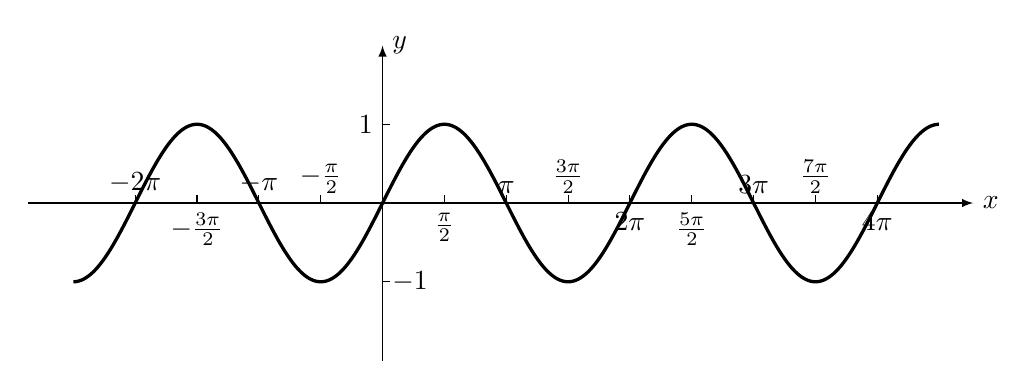
\begin{tikzpicture}[>=latex, xscale=.5]
\draw[->](-9,0)--(15,0)node[right]{$x$}; 
\draw [->](0,-2)--(0,2)node[right]{$y$};
    
\draw[domain=-2.5*pi : pi*4.5,  samples=2000, very thick] plot(\x, {sin(\x r)});

\foreach \x in {-4,-3,...,8}
{
    \draw (\x/2*pi,0)--(\x/2*pi,0.1);
}
\node at (-2*pi,0)[above]{$-2\pi$};
\node at (-1.5*pi,0)[below]{$-\frac{3\pi}{2}$};
\node at (-1*pi,0)[above]{$-\pi$};
\node at (-.5*pi,0)[above]{$-\frac{\pi}{2}$};
\node at (.5*pi,0)[below]{$\frac{\pi}{2}$};
\node at (1*pi,0)[above]{$\pi$};
\node at (1.5*pi,0)[above]{$\frac{3\pi}{2}$};
\node at (2*pi,0)[below]{${2\pi}$};
\node at (2.5*pi,0)[below]{$\frac{5\pi}{2}$};    
\node at (3*pi,0)[above]{$3\pi$};
\node at (3.5*pi,0)[above]{$\frac{7\pi}{2}$};
\node at (4*pi,0)[below]{$4\pi$};


\draw (0,1)--(.2,1);
\draw (0,-1)--(.2,-1);
\node at (0,1)[left]{1};
\node at (0,-1)[right]{$-1$};



\end{tikzpicture}
    \caption{}
\end{figure}

因此,在精确度要求不太高时,我们常用“五点法”作出关于正弦函数在$[0, 2\pi]$上的图象。

\begin{example}
    用五点法作出$y=1+\sin x,\quad x\in [0, 2\pi]$的图象。
\end{example}

\begin{solution}
    列表    
\begin{center}
\begin{tabular}{c|ccccc}
    \hline
    $x$ & 0  & $\frac{\pi}{2}$  & $\pi$  & $\frac{3\pi}{2}$  & $2\pi$  \\
    \hline
    $\sin x$   &  0 & 1  & 0  & $-1$  &0\\
    $1+\sin x$   & 1  & 2  & 1  & 0  & 1\\
    \hline
\end{tabular}    
\end{center}

描点作图:(如图7.3)
\begin{figure}[htp]
    \centering
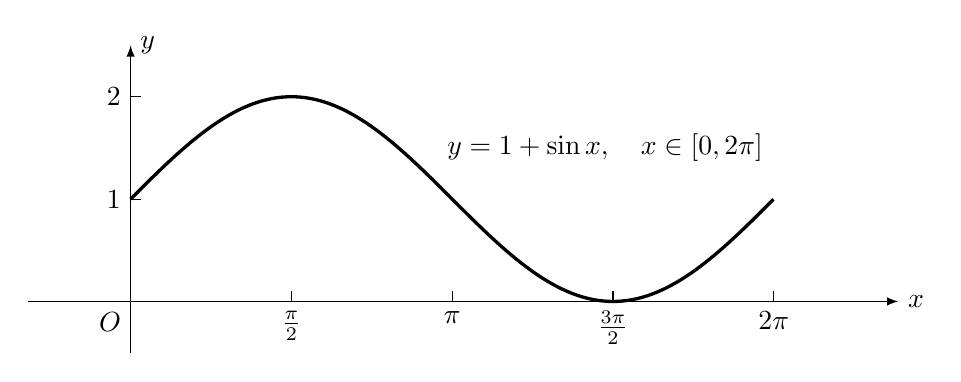
\begin{tikzpicture}[>=latex, scale=1.3]
\draw[->](-1,0)--(7.5,0)node[right]{$x$}; 
\draw [->](0,-.5)--(0,2.5)node[right]{$y$};
    
\draw[domain=0 :2*pi,  samples=1000, very thick] plot(\x, {sin(\x r)+1});
\foreach \x in {1,...,4}
{
    \draw (\x/2*pi,0)--(\x/2*pi,.1);
}
\node at (0,1)[left]{1};
\node at (0,2)[left]{$2$};
\draw (0,1)--(.1,1);
\draw (0,2)--(.1,2);

\node at (-.2,-.2){$O$};
\node at (1/2*pi,0)[below]{$\frac{\pi}{2}$};
\node at (pi,0)[below]{$\pi$};
\node at (3/2*pi,0)[below]{$\frac{3\pi}{2}$};
\node at (2*pi,0)[below]{$2\pi$};

\node at (3,1.5)[right]{$y=1+\sin x,\quad x\in [0,2\pi]$};

\end{tikzpicture}
    \caption{}
\end{figure}

\end{solution}

我们也可以用几何法作出$[0, 2\pi]$上正弦函数的图象。如图7.4所示,在$O-x$轴的负半轴上任意取一点,以这点为圆心,单位长为半径作圆,从这个圆的右半圆和$O-x$轴的交点$P_0$量起,把这个圆分成12等份,并在$O-x$轴上,从原点起向右取长等于$2\pi$(即单位圆的周长)的一段,也分成12等份,过圆上的各个分点,分别向$Ox$轴作垂线,便得到各分点上的纵坐标,显然,这些点的纵坐标就是对应各角(数)的正弦值,因此过各分点作平行于$O-x$轴的直线,它们分别与由$O-x$轴上各个对应点处所作$Ox$轴的垂线相交,这些交点就是$y=\sin x$图象上的点。把这些点依次连结成平滑的曲线,就得到正弦函数$y=\sin x$在$[0, 2\pi]$区间上的图象。

如果把曲线在$[0, 2\pi]$间的一段,沿着$Ox$轴向左、右连续移动,每次移动$2\pi$个单位,就可以得到如图7.2所示的连续不断的正弦曲线。

\begin{figure}[htp]
    \centering
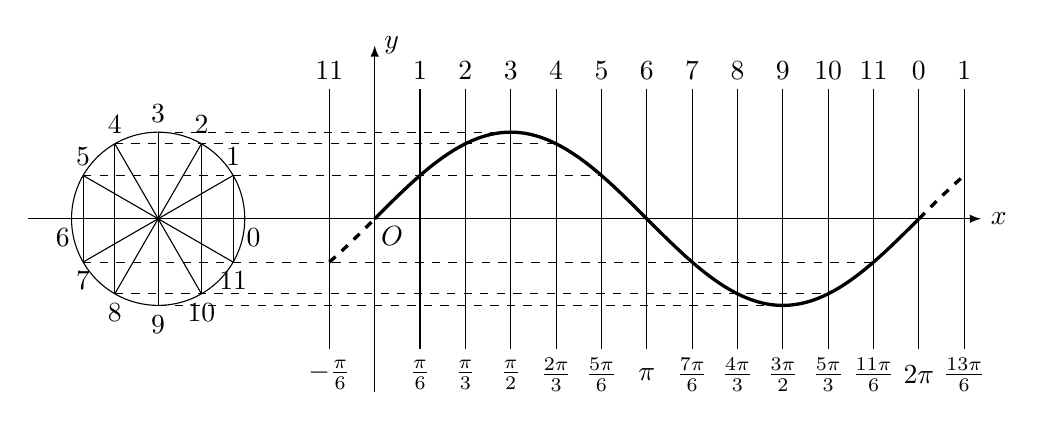
\begin{tikzpicture}[>=latex,scale=1.1]

\draw[->] (-4,0)--(7,0)node[right]{$x$};
\draw [->](0,-2)--(0,2)node[right]{$y$};
\draw (-2.5,0) circle (1);

\draw[domain=0 : pi*2,  samples=1000, very thick] plot(\x, {sin(\x r)});

\foreach \x in {1,2,...,11}
{
    \draw (\x*pi/6,1.5)node[above]{\x}--(\x*pi/6,-1.5);
}

\foreach \x in {1,2,...,5}
{
    \draw (-2.5,0)--+ (\x*30:1)node[above]{\x};
}
\foreach \x in {7,8,...,11}
{
    \draw (-2.5,0)--+ (\x*30:1)node[below]{\x};
}



\draw (-2.5+.5, .5*1.732)--(-2.5+.5, -.5*1.732);
\draw (-2.5-.5, .5*1.732)--(-2.5-.5, -.5*1.732);
\draw (-2.5-.5*1.732, .5)--(-2.5-.5*1.732, -.5);
\draw (-2.5+.5*1.732, .5)--(-2.5+.5*1.732, -.5);
\draw [dashed] (-2.5-.5, .5*1.732)--(2*pi/3, .5*1.732);
\draw [dashed] (-2.5-.5*1.732, .5)--(5*pi/6, .5);
\draw [dashed] (-2.5-.5, -.5*1.732)--(5*pi/3, -.5*1.732);
\draw [dashed] (-2.5-.5*1.732, -.5)--(11*pi/6, -.5);

\draw[dashed] (-2.5, 1)--(pi/2, 1);
\draw [dashed](-2.5, -1)--(1.5*pi, -1);
\node at (-1*pi/6,-1.8){$-\frac{\pi}{6}$};
\node at (13*pi/6,-1.8){$\frac{13\pi}{6}$};
\node at (1*pi/6,-1.8){$\frac{\pi}{6}$};
\node at (2*pi/6,-1.8){$\frac{\pi}{3}$};
\node at (3*pi/6,-1.8){$\frac{\pi}{2}$};
\node at (4*pi/6,-1.8){$\frac{2\pi}{3}$};
\node at (5*pi/6,-1.8){$\frac{5\pi}{6}$};
\node at (6*pi/6,-1.8){$\pi$};
\node at (7*pi/6,-1.8){$\frac{7\pi}{6}$};
\node at (8*pi/6,-1.8){$\frac{4\pi}{3}$};
\node at (9*pi/6,-1.8){$\frac{3\pi}{2}$};
\node at (10*pi/6,-1.8){$\frac{5\pi}{3}$};
\node at (11*pi/6,-1.8){$\frac{11\pi}{6}$};
\node at (12*pi/6,-1.8){$2\pi$};

\draw (-pi/6,1.5)node[above]{11}--(-pi/6,-1.5);
\draw (2*pi,1.5)node[above]{0}--(2*pi,-1.5);
\draw (13*pi/6,1.5)node[above]{1}--(13*pi/6,-1.5);

\draw[domain=-pi/6: 0,  samples=100, very thick, dashed] plot(\x, {sin(\x r)});
\draw[domain=pi*2:13*pi/6,  samples=100, very thick, dashed] plot(\x, {sin(\x r)});

\node at (-1.4, 0)[below]{0};
\node at (-3.6, 0)[below]{6};

\node at (.2,-.2){$O$};
\end{tikzpicture}
    \caption{}
\end{figure}

\begin{ex}
    \begin{enumerate}
        \item 作$y=|\sin x|,\quad x\in\mathbb{R}$的图象。
        \item 用“五点法”作出下列各函数的图象($0\le x\le 2\pi$), 并且和$y=\sin x$的图象比较,说明这些图象 和$y=\sin x$的图象的区别。
        \begin{enumerate}
            \item $y=\sin x-1$
            \item $y=1-\sin x$
          \item $y=2\sin x$
        \end{enumerate}
    \end{enumerate}
\end{ex}

\subsection{正弦函数的主要性质}

由上一章的讨论和正弦函数图象,我们可以得到正弦函数$y=\sin x$的主要性质如下:
\begin{enumerate}
    \item 定义域\quad 正弦函数的定义域是一切实数,也就是说,当自变量$x$取任何实数值时,正弦函数$y$都有唯一确定的值与之对应,从图象上看曲线随着$x$轴连续不断地无限延伸。
    \item 值域\quad 由图7.2看出,曲线上点的纵坐标最小是-1,最大是1,正弦函数值是在$-1$与$+1$之间,这说明正
    弦函数的值域是闭区间$[-1, 1]$, 或$|\sin x|\le 1$.
    \item 奇偶性\quad 正弦函数是奇函数,因此,正弦曲线关于原点对称。
    \item 函数的符号\quad 终边落在$x$轴的上半平面时,正弦函数为正;落在轴的下半平面时,正弦函数为负。也就是说,在区间$(0,\pi)$内,$\sin x>0$。 一般地,当$2k\pi <x<(2k+1)\pi$时($k\in\mathbb{Z}$),$\sin x>0$。在区间$(\pi,2\pi)$内,$\sin x<0$. 一般地,当$(2k+1)\pi<x<2(k+1)\pi$时,$\sin x<0$。这反映在图象上,在区间$(2k\pi, (2k+1)\pi),\;\; k=0,\pm1,\pm2,\ldots$上,曲线在$x$轴的上方;在区间$((2k+1)\pi, 2(k+1)\pi),\;\; k=0,\pm1,\pm2,\ldots$上,曲线在$x$轴下方。
    
    当横坐标$x=0$, $x=\pi$和$x=2\pi$时,正弦函数值为零.一般地,当$x=k\pi\; (k\in \mathbb{Z})$时,$\sin x=0$, 这时曲线与$x$轴相交.

    \item 增减性\quad 由正弦曲线容易看出,随着$x$增加正弦函数在区间$\left(-\frac{\pi}{2},\frac{\pi}{2}\right)$内是递增的;在区间$\left(-\frac{\pi}{2},\frac{3\pi}{2}\right)$内是递减的。一般的情况是$\sin x$在区间$\left(-\frac{\pi}{2}+2k\pi,\frac{\pi}{2}+2k\pi\right)$内是递增的,在区间$\left(\frac{\pi}{2}+2k\pi,\frac{\pi}{2}+(2k+1)\pi\right)$内是递减的,这里$k\in \mathbb{Z}$。
    
    由$\sin x$的增减性看出,在$x=\frac{\pi}{2}$一处,正弦函数由递增变为递减,因此在$x=\frac{\pi}{2}$处,$\sin x$取得极大值1. 一般地,当$x=\frac{\pi}{2}+2k\pi\;\; (k\in\mathbb{Z})$时,$\sin x=1$是极大值。同时还看
    出,在$x=\frac{3\pi}{2}$处,正弦函数由递减变为递增,因此在
    $x=\frac{3\pi}{2}$处,$\sin x$取得极小值$-1$, 一般地,当
    $x=\frac{3\pi}{2}+2k\pi\;\; (k\in\mathbb{Z})$
    时,$\sin x=-1$是极小值。
    \item 周期性\quad 当横坐标$x$每隔$2\pi$ 时,曲线重复出现,也就是说,正弦曲线上任何一点的横坐标加上或减去$2\pi$ 时,对应的纵坐标相等,即
\[\sin(x\pm 2\pi)=\sin x\]
一般地:
\[\sin(x+2k\pi)=\sin x\quad (k\in\mathbb{Z})\]

从上面的公式知道正弦函数是周期函数,它的周期有无穷多个,即$2\pi$ 的整数倍,但是我们所关心的是最小正周期。

下面我们来研究一般的周期函数的定义,并证明正弦函数的最小正周期是$2\pi$。
\end{enumerate}

\begin{blk}{定义}
    设有$x$的函数$f(x)$, 若存在不等于0的一个常
数$p$, 使对于函数定义域中的任何实数$x$, 等式
\begin{equation}
    f (x) =f (x+p) 
\end{equation}
成立,则称$f(x)$是周期函数,常数$p$叫做函数$f(x)$的一个周期。
\end{blk}

下面我们来说明,任何周期函数一定有正周期。

在等式(7.1)中,以$x-p$替换$x$, 就得到
\[f (x-p) =f (x)\]
因此有$f (x) =f (x\pm p)$。这也就是说,$\pm p$都是函数$f(x)$的周期,故$f(x)$必有正周期。

函数$f(x)$的最小正周期应满足:
\begin{enumerate}
    \item $p>0$;
    \item 对于任意实数$x$, 正数$p$须使$f(x+p)=f(x)$成立;
    \item $p$为满足1、2的最小正数。
\end{enumerate}

下面我们来证明$\sin x$的最小正周期等于$2\pi$。

在恒等式 $\sin(x+p)=\sin x$ 中,令$x=0$, 得到$\sin p=0$,
在单位圆上,弧的始点为$(1, 0)$, 而弧长分别等于0和$\pi$的这两个弧的端点$P_0,P_{\pi}$的纵坐标等于0, 又和这两个点对应的最小正数分别是$2\pi$和$\pi$。在这两个数中,$\pi$显然不能是周期,因为,$\sin\frac{\pi}{2}=1$,但$\sin\left(\frac{\pi}{2}+\pi\right)=-1$
,因此最小
正周期只可能是$2\pi$, 由于$\sin(x+2\pi)=\sin x$, 对于任何数$x$都成立,所以$\sin x$的最小正周期等于$2\pi$。

\begin{example}
    求下列函数的最小正周期:
\begin{multicols}{2}
\begin{enumerate}
    \item $y=\sin2x $ 
    \item $y=2\sin\left(4x-\frac{\pi}{6}\right)$
\end{enumerate}
\end{multicols}
\end{example}

\begin{solution}
\begin{enumerate}
\item
    因为 $\sin2x =\sin(2x+2\pi)=\sin 2(x+\pi), \;\; (x\in\mathbb{R})$, 即当自变量$x$改变成$x+\pi$时,函数值不变,所以$y=\sin2x$的周期$T=\pi$.

为证明$\pi$是$\sin2x$的最小正周期,我们用反证法。假设$y=\sin2x$还有一个比$\pi$小的正周期$T'$, 即$0<T'<\pi$,根据周期$T'$的定义,我们有
\[\sin2 (x+T') =\sin2x\]
即
$$\sin (2x+2T') =\sin2x$$
令$x=0$, 代入上式得$\sin 2T'=0$,
依不等式$0<T'<\pi$,从而$0<2T'<2\pi$,得到$2T'=\pi$
即
\[T'=\frac{\pi}{2}\]

今验知,$\sin2\left(x+\frac{\pi}{2}\right)=\sin(2x+\pi)=-\sin2x$. 故$T'$不是$y=\sin2x$的周期,因此得到矛盾。这就是说 $\sin 2x$的最小正周期是$\pi$。



\item 由于:
\[\begin{split}
    2\sin\left(4x-\frac{\pi}{6}\right)&=2\sin\left(4x-\frac{\pi}{6}+2\pi\right)\\
    &=2\sin\left[4\left(x+\frac{\pi}{2}\right)-\frac{\pi}{6}\right]\quad (x\in\mathbb{R})
\end{split}\]
即当自变量$x$改变成$x+\frac{\pi}{2}$时,函数值不变,所以$y=
2\sin\left(4x-\frac{\pi}{8}\right)$的周期$T=\frac{\pi}{2}$. 再证$T=\frac{\pi}{2}$是$y=2\sin\left(4x-\frac{\pi}{8}\right)$的最小正周期。

假设$y=2\sin\left(4x-\frac{\pi}{8}\right)$还有一个比$\frac{\pi}{2}$小的正周期
$T'$,即$0<T'<\frac{\pi}{2}$,
从而得到
\begin{equation}
    0<4T'<2\pi
\end{equation}

根据周期$T'$的定义,我们有
\begin{equation}
    2\sin \left[4(x+T')-\frac{\pi}{6}\right]=2\sin \left(4x-\frac{\pi}{6}\right)
\end{equation}
即
\begin{equation}
    2\sin \left[\left(4x-\frac{\pi}{6}\right)+4T'\right]=2\sin \left(4x-\frac{\pi}{6}\right)
\end{equation}

令 $4x-\frac{\pi}{6}=0$, 即$x=\frac{\pi}{24}$, 代入(7.4), 得
$$2\sin 4T'=0$$
依不等式(7.2),$4T'$的值只能是$\pi$,即$T'=\frac{\pi}{4}$。今验证知
\[2\sin\left[4\left(x+\frac{\pi}{4}\right)-\frac{\pi}{6}\right]=2\sin \left(4x+\pi-\frac{\pi}{6}\right)=-2\sin\left(4x-\frac{\pi}{6}\right)\]
故$T'=\frac{\pi}{4}$不是$2\sin\left(4x-\frac{\pi}{6}\right)$的周期,因此得到矛盾。这就证明了$y=2\sin\left(4x-\frac{\pi}{6}\right)$的最小正周期是$\frac{\pi}{2}$。
\end{enumerate}
\end{solution}

一般地,对于函数$y=A\sin(\omega x+\varphi)$ ($\omega,\varphi$为常数,且$\omega\ne 0$, $x\in\mathbb{R}$),由于
\[\begin{split}
    A\sin(\omega x+\varphi)&=A\sin(\omega x+\varphi+2\pi)\\
    &=A\sin\left[\omega\left(x+\frac{2\pi}{\omega}\right)+\varphi\right]  
\end{split}\]
故$\frac{2\pi}{|\omega|}$是$y=A\sin(\omega x+\varphi)$的一个正周期,它只与自变量的系数有关,而与$A,\varphi$无关。用上面同样的方法可以证明$\frac{2\pi}{|\omega|}$是$y=A\sin(\omega x+\varphi)$的最小正周期(证明留给读者去完成)。

\begin{example}
不求值决定下列各差的符号:
\begin{enumerate}
    \item $\sin 20^{\circ}12'-\sin20^{\circ}13'$
    \item $\sin\left(-\frac{\pi}{18}\right)-\sin\left(-\frac{\pi}{10}\right)$
    \item $ \sin1605^{\circ}-\sin1657^{\circ}$
\end{enumerate}  
\end{example}

\begin{solution}
\begin{enumerate}
    \item 正弦函数在第一象限是增函数,
    
$\therefore\quad  \sin 20^{\circ}12'<\sin20^{\circ}13'$
即
    \[\sin 20^{\circ}12'-\sin20^{\circ}13'<0\]
\item $\because\quad -\frac{\pi}{2}<-\frac{\pi}{10}<-\frac{\pi}{18}<\frac{\pi}{2}$

正弦函数$y=\sin x$在$-\frac{\pi}{2}<x<\frac{\pi}{2}$上是增函数

$\therefore\quad \sin\left(-\frac{\pi}{10}\right)<\sin\left(-\frac{\pi}{18}\right)$
即
\[\sin\left(-\frac{\pi}{18}\right)-\sin\left(-\frac{\pi}{10}\right)>0\]

\item $\because\quad \sin 1605^{\circ}=\sin 165^{\circ},\qquad \sin 1657^{\circ}=\sin 217^{\circ}$

又$\because\quad 90^{\circ}<165^{\circ}<217^{\circ}<270^{\circ}$,正弦函数$y=\sin x$在$90^{\circ}<x<270^{\circ}$上是减函数。

$\therefore\quad \sin 165^{\circ}>\sin 217^{\circ}$,即
\[\sin 1605^{\circ}-\sin 1657^{\circ}>0\]
\end{enumerate}
\end{solution}

\begin{example}
    求证定圆的外切菱形中以正方形的面积最小。
\end{example}

\begin{solution}
如图7.5, 设定圆$O$的半径为$r$, 它的外切菱形中的$\angle A=\theta$, 由于对边切点连线必过圆心,故外切菱形的高等于$2r$, 外切菱形的边长为$\frac{2r}{\sin\theta}$。

\begin{figure}[htp]
    \centering
    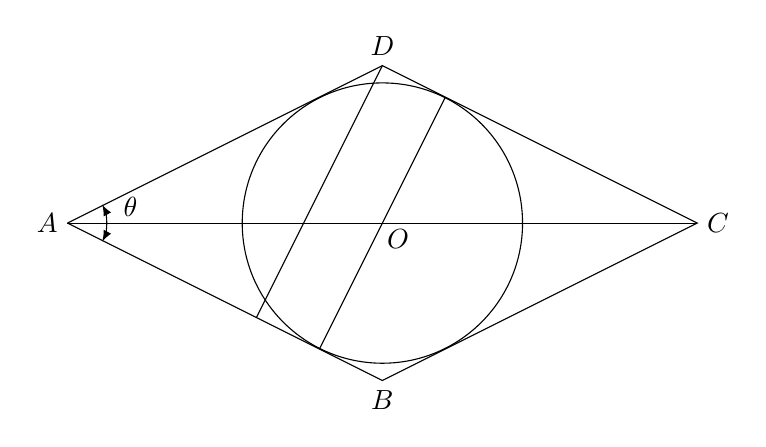
\begin{tikzpicture}[>=latex]
 \draw (-4,0)node[left]{$A$}--(0,2)node[above]{$D$}--(4,0)node[right]{$C$}--(0,-2)node[below]{$B$}--(-4,0)    ;
\draw (-4,0)--(4,0);
\draw (0,0) circle (1.78);       
\draw (.8,1.6)--(-.8,-1.6);
\draw (0,2)--(-1.6,-1.2);
\node at (.2,-.2){$O$};
\draw[->](-3.5,0) arc (0:28:.5);
\draw[->](-3.5,0) arc (0:-28:.5);
\node at (-3.2,0.2){$\theta$};
    \end{tikzpicture}
    \caption{}
\end{figure}

    于是,菱形面积$S=2r\cdot \frac{2r}{\sin\theta}$,当$\sin\theta=1$时,菱形面积$S$最小,这时$\theta=90^{\circ}\;\;(0^{\circ}<0<180^{\circ})$.
    
因此,定圆的外切菱形中以正方形的面积最小。
\end{solution}

\begin{example}
求函数$y=\left(\sin x-\frac{1}{2}\right)^2+2$的最大值和最小值,
并求取最大值或最小值时的$x$值。
\end{example}

\begin{solution}
    把$y$看作$\sin x$的二次函数,这样问题变成求闭区间$-1\le \sin x\le 1$上的$y$的最大值和最小值。也就是要把开区间$(-1, 1)$内的极值和两端点处的函数值作比较。

\begin{enumerate}
    \item 当$\sin x=-1$时,$y=\left(-1-\frac{1}{2}\right)^2+2=4\frac{1}{4}$
    \item 当$\sin x=1$时,$y=\left(1-\frac{1}{2}\right)^2+2=2\frac{1}{4}$
    \item 当$\sin x=\frac{1}{2}$时,极小值$y=2$, 这是函数在$(-1, 1)$中的唯一极值点。
\end{enumerate}

因此,
\begin{enumerate}
    \item 当$\sin x=-1$, 即$x=-\frac{\pi}{2}+2k\pi\quad (k\in\mathbb{Z})$时,
最大值$y=4\frac{1}{4}$;
\item 当$\sin x=\frac{1}{2}$,即$x=\frac{\pi}{6}+2k\pi$或$\frac{5\pi}{6}+2k\pi \quad (k\in\mathbb{Z})$时,
最小值$y=2$。
\end{enumerate}


\end{solution}


\section*{习题7.1}
\addcontentsline{toc}{subsection}{习题7.1}
\begin{enumerate}
    \item 比较下列各组中两个三角函数值的大小(不求值):
    \begin{enumerate}
        \item $\sin250^{\circ}$和$\sin260^{\circ}$
        \item $\sin\left(-\frac{54}{7}\pi\right)$和$\sin\left(-\frac{63}{8}\pi\right)$
        \item $\sin380^{\circ}$和 $\sin480^{\circ}$
    \end{enumerate}
    
    \item 说出下列各函数的最小正周期:
\begin{multicols}{2}
    \begin{enumerate}
        \item $y=\sin 3x$
        \item $y=\sin\frac{x}{2}$
        \item $y=\sin \left(x+\frac{\pi}{3}\right)$
        \item $y=\cos \left(2 x-\frac{\pi}{6}\right)$
        \item $y=3 \sin \left(\frac{x}{3}+\frac{\pi}{4}\right)$
        \item $y=3 \sin \left(\pi x+\frac{\pi}{3}\right)+1$
    \end{enumerate}
\end{multicols}

\item 求下列函数的最大值和最小值,又在何时有最大值
或最小值:
\begin{multicols}{2}
    \begin{enumerate}
\item $y=|\sin x|$
\item $y=1+\sin x$
\item $y=1+5 \sin ^{2} x$
\item $y=\frac{1}{1-\sin x}$
\item $y=\left(\sin x-\frac{3}{2}\right)^{2}-2 $
\item $y=2-\left(\sin x-\frac{\sqrt{3}}{2}\right)^{2}$
    \end{enumerate}
\end{multicols}

\item 求证等腰三角形中,若腰长一定则等腰直角三角形
的面积最大。
\item $y=|\sin x|$是周期函
数吗?如果是,说出它的最小正周期。
\item 作$y=\sin|x|$的图象,试从它的图象说明函数$y=\sin|x|$不是周期函数:

\item 利用单位圆,容易看出$\sin x<\frac{1}{2}$的解的范围,如下图所示。
\[\frac{5\pi}{6}+2k\pi<x<\frac{\pi}{6}+2(k+1)\pi\]
\begin{center}
\begin{tikzpicture}[>=latex, scale=1.5]

\draw [thick] (0,0) circle (1);

\draw[->] (-1.5,0)--(2,0)node[right]{$x$};
\draw[->] (0,-1.5)--(0,2)node[right]{$y$};    
\draw (1.732/2,.5)--(-1.732/2,.5);
\node at (0,.55)[right]{$(0,\tfrac{1}{2})$};
\foreach \x in {15,30,150,165}
{
    \draw (0,0)--(\x:1);
}
\foreach \x in {198,216,...,342}
{
    \draw (0,0)--(\x:1);
}

\node at (30:1)[right]{$P_{\tfrac{\pi}{6}}$};
\node at (150:1)[left]{$P_{\tfrac{5\pi}{6}}$};


\end{tikzpicture}    
\end{center}


用同样的方法解下面不等式:
\[\sin 2x>\frac{1}{2},\qquad \sin 3x\ge -\frac{\sqrt{2}}{2}\]
\end{enumerate}  

\section{余弦函数的图象和性质}
\subsection{余弦函数的图象}

我们知道余弦函数的定义域是$(-\infty,+\infty)$, 它是个偶函数,故它的图象向$x$轴的正负方向无限延伸,图象关于$y$轴对称。

我们从第五章中知道,函数$f(x+\ell)$的图象是由函数$f(x)$的图象向左、右平移$|\ell|$个单位得到,当$\ell>0$时,向左平移1个单位,当$\ell<0$时,向右平移$|\ell|$个单位。

在上一章我们又知道,$\cos x=\sin\left(\frac{\pi}{2}+x\right)$,
故$y=\cos x$的
图象就是$y=\sin\left(x+\frac{\pi}{2}\right)$的图象,而正弦型函数$y=\sin\left(x+\frac{\pi}{2}\right)$的图象恰是正弦函数$y=\sin x$的图象向左
平移$\frac{\pi}{2}$个单位得到,这就是说,我们只须把正弦曲线
$y=\sin x$沿着$x$轴向左平移$\frac{\pi}{2}$个单位就得到余弦函数$y=\cos x$
的图象。如图7.6所示。

 \begin{figure}[htp]
     \centering
     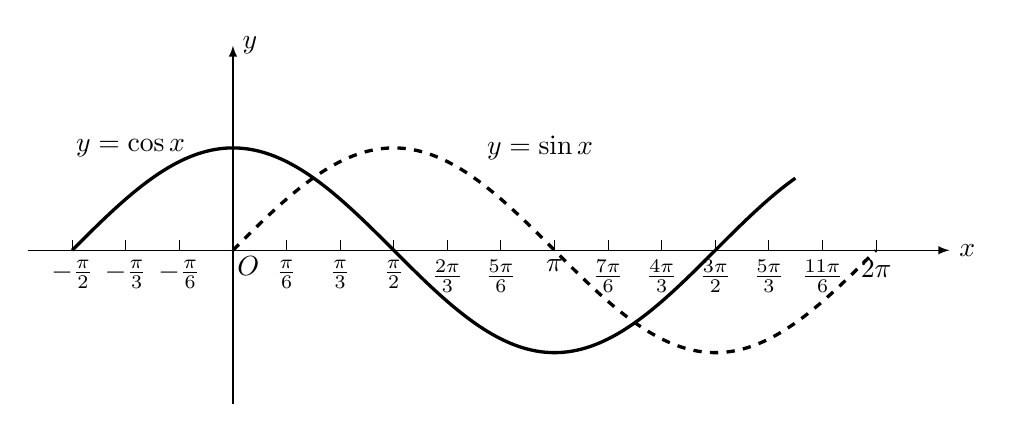
\begin{tikzpicture}[scale=1.3, >=latex]

\draw[->] (-2,0)--(7,0)node[right]{$x$};
\draw [->](0,-1.5)--(0,2)node[right]{$y$};
\draw[domain=0 : pi*2,  samples=1000, very thick, dashed] plot(\x, {sin(\x r)});
\draw[domain=-0.5*pi : pi*1.75,  samples=1000, very thick] plot(\x, {cos(\x r)});

\foreach \x in {-3,-2,...,12}
{
    \draw (\x*pi/6, 0)--(\x*pi/6, .1);
}
\node at (-1,1){$y=\cos x$};  \node at (3,1){$y=\sin x$};

\node at (-3*pi/6, 0)[below]{$-\frac{\pi}{2}$};
\node at (-2*pi/6, 0)[below]{$-\frac{\pi}{3}$};
\node at (-1*pi/6, 0)[below]{$-\frac{\pi}{6}$};
\node at (1*pi/6, 0)[below]{$\frac{\pi}{6}$};
\node at (2*pi/6, 0)[below]{$\frac{\pi}{3}$};
\node at (3*pi/6, 0)[below]{$\frac{\pi}{2}$};
\node at (4*pi/6, 0)[below]{$\frac{2\pi}{3}$};
\node at (5*pi/6, 0)[below]{$\frac{5\pi}{6}$};
\node at (6*pi/6, 0)[below]{$\pi$};
\node at (7*pi/6, 0)[below]{$\frac{7\pi}{6}$};
\node at (8*pi/6, 0)[below]{$\frac{4\pi}{3}$};
\node at (9*pi/6, 0)[below]{$\frac{3\pi}{2}$};
\node at (10*pi/6, 0)[below]{$\frac{5\pi}{3}$};
\node at (11*pi/6, 0)[below]{$\frac{11\pi}{6}$};
\node at (12*pi/6, 0)[below]{$2\pi$};
\node at (.15,-.15){$O$};
     \end{tikzpicture}
     \caption{}
 \end{figure}

 当然,也可以用描点法来作余弦函数的图象。根据上面所说的我们可以借助第一节中的正弦函数值表,将自变数$x$的取值分别减去$\frac{\pi}{2}$
 而对应的$y$值仍不变就能够得到余弦函数
 值表。

 把表内$x$、$y$的每一对值作为点的坐标,在直角坐标系内作出对应的点,将它们依次连结成平滑曲线,这样就得到余弦函数在$\left[\frac{\pi}{2},\frac{3\pi}{2}\right]$上的图象。如果把曲线$\left[\frac{\pi}{2},\frac{3\pi}{2}\right]$
 上的一段,沿着$x$轴向左、右推移,每次移动$2\pi$个单
 位,就可以得到连续不断的余弦函数的图象(图7.7)。

\begin{center}
\begin{tabular}{c|ccccccc}
    \hline
$x$ & $-\frac{\pi}{2}$& $-\frac{\pi}{3}$& $-\frac{\pi}{6}$& 0 & $\frac{\pi}{6}$& $\frac{\pi}{3}$& $\frac{\pi}{2}$\\
$y=\cos x$ & 0  & $\frac{1}{2}$  & $\frac{\sqrt{3}}{2}$  & 1  & $\frac{\sqrt{3}}{2}$  & $\frac{1}{2}$ & 0\\
\hline
$x$ && $\frac{2\pi}{3}$& $\frac{5\pi}{6}$& $\pi$& $\frac{7\pi}{6}$& $\frac{4\pi}{3}$&$\frac{3\pi}{2}$\\
$y=\cos x$ && $-\frac{1}{2}$  & $-\frac{\sqrt{3}}{2}$  & $-1$  & $-\frac{\sqrt{3}}{2}$  & $-\frac{1}{2}$  & 0\\
\hline
\end{tabular}
\end{center}

\begin{figure}[htp]
    \centering
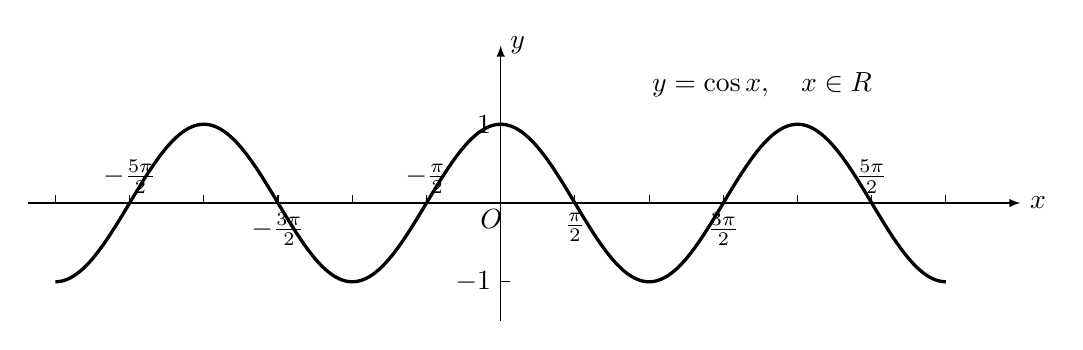
\begin{tikzpicture}[>=latex, xscale=.6]
\draw[->](-10,0)--(11,0)node[right]{$x$}; 
\draw [->](0,-1.5)--(0,2)node[right]{$y$};
    
\draw[domain=-3*pi :3*pi,  samples=2000, very thick] plot(\x, {cos(\x r)});
\foreach \x in {-3,-2.5,...,3}
{
    \draw (\x*pi,0)--(\x*pi,.1);
}

\foreach \x in {1,-1}
{
    \draw (0,\x)node[left]{$\x$}--(.2,\x);
}


\node at (-.2,-.2){$O$};
\node at (-2.5*pi,0)[above]{$-\frac{5\pi}{2}$};
\node at (-.5*pi,0)[above]{$-\frac{\pi}{2}$};
\node at (2.5*pi,0)[above]{$\frac{5\pi}{2}$};
\node at (-1.5*pi,0)[below]{$-\frac{3\pi}{2}$};
\node at (.5*pi,0)[below]{$\frac{\pi}{2}$};
\node at (1.5*pi,0)[below]{$\frac{3\pi}{2}$};

\node at (3,1.5)[right]{$y=\cos x,\quad x\in \mathbb{R}$};

\end{tikzpicture}
    \caption{}
\end{figure}

余弦函数$y=\cos x$的图象叫做余弦曲线。

如作正弦函数的图象那样,只要把$\left(-\frac{\pi}{2},0\right)$、$(0, 1)$、$\left(\frac{\pi}{2},0\right)$、$(\pi,-1)$、$\left(\frac{3\pi}{2},0\right)$这五个点作出后,余弦函数$y=\cos x,\;\; x\in\left[-\frac{\pi}{2},\frac{3\pi}{2}\right]$的图象就基本确定了。因此,
在精确度要求不太高的情况下,也可用“五点法”作出关于余弦函数的图象。

\begin{example}
 用“五点法”作出$y=-\cos x,\;\; x\in[0,2\pi]$ 的图象。   
\end{example}

\begin{solution}
    列表并作图(如图7.8所示)
\begin{center}
\begin{tabular}{cccccc}
\hline
    $x$  &0&$\frac{\pi}{2}$&$\pi$&$\frac{3\pi}{2}$&$2\pi$\\
    \hline
   $\cos x$&1&0&$-1$&0&1\\ 
$-\cos x$&$-1$&0&1&0&$-1$\\
\hline
\end{tabular}    
\end{center}

\begin{figure}[htp]
    \centering
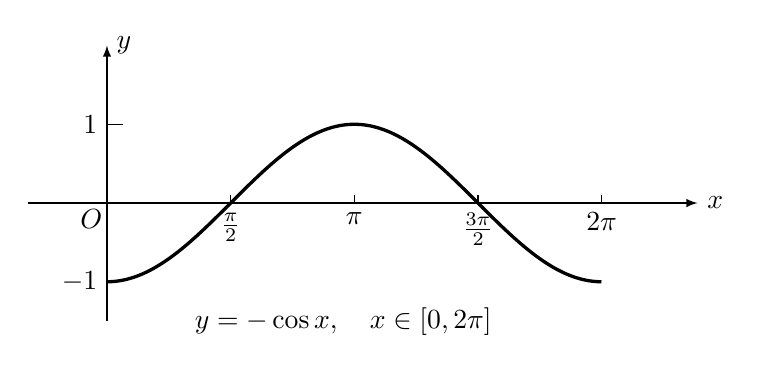
\begin{tikzpicture}[>=latex, xscale=1]
\draw[->](-1,0)--(7.5,0)node[right]{$x$}; 
\draw [->](0,-1.5)--(0,2)node[right]{$y$};
    
\draw[domain=0:2*pi,  samples=1000, very thick] plot(\x, {-cos(\x r)});
\foreach \x in {1,2,...,4}
{
    \draw (\x*pi/2,0)--(\x*pi/2,.1);
}

\foreach \x in {1,-1}
{
    \draw (0,\x)node[left]{$\x$}--(.2,\x);
}


\node at (-.2,-.2){$O$};
\node at (.5*pi,0)[below]{$\frac{\pi}{2}$};
\node at (1*pi,0)[below]{$\pi$};
\node at (1.5*pi,0)[below]{$\frac{3\pi}{2}$};
\node at (2*pi,0)[below]{$2\pi$};

\node at (3,-1.5){$y=-\cos x,\quad x\in [0,2\pi]$};

\end{tikzpicture}
    \caption{}
\end{figure}
\end{solution}

\subsection{余弦函数的主要性质}

由上一章的讨论和余弦函数图象,我们可以得到余弦函数$y=\cos x$的主要性质如下:
\begin{enumerate}
\item 定义域\quad  余弦函数$y=\cos x$的定义域是一切实数,即$-\infty<x<+\infty$或$(-\infty, +\infty)$;
\item 值域\quad 余弦函数$y=\cos x$的值域是$[-1, 1]$, 或
$|\cos x|\le 1$;
\item 奇偶性\quad 余弦函数是偶函数;
\item 函数的符号
\begin{itemize}
    \item 当$-\frac{\pi}{2}+2k\pi<x<\frac{\pi}{2}+2k\pi$时,$\cos x>0$;
    \item 当$\frac{\pi}{2}+2k\pi<x<\frac{\pi}{2}+(2k+1)\pi$时,$\cos x<0$;
    \item 当$x=\frac{\pi}{2}+k\pi$时,$\cos x=0$,这里$k\in\mathbb{Z}$。
\end{itemize}

\item 增减性
\begin{itemize}
    \item $y=\cos x$在区间$[2k\pi,(2k+1)\pi]$内是递减的;
    \item $y=\cos x$在区间$[(2k+1)\pi,2(k+1)\pi]$内是递增的。
\end{itemize}
因此,
\begin{itemize}
    \item 当$x=2k\pi$时,$\cos x=1$是极大值。
    \item 当$x=(2k+1)\pi$时,$\cos x=-1$是极小值,这里$k\in\mathbb{Z}$。
\end{itemize}

\item 周期性\quad 余弦函数$y=\cos x$的最小正周期(以后简称周期)是$2\pi$。

函数$y=\cos x$的周期是$\frac{2\pi}{|\omega|}\quad (\omega\ne 0,\;\;x\in \mathbb{R})$一般地,函数$y=A\cos(\omega x+\varphi)$的周期是$\frac{2\pi}{|\omega|}$
($\omega,\varphi$为常数,且$\omega\ne 0,\;\;x\in \mathbb{R}$)。

因为$\cos(\omega x+\varphi)=\sin\left[\omega x+\left(\varphi+\frac{\pi}{2}\right)\right]$, 这里$\omega$是不等于0的常数,$\varphi+\frac{\pi}{2}$仍是常数,根据函数$y=A\sin\left[\omega x+\left(\varphi+\frac{\pi}{2}\right)\right]$的最小正周期是$\frac{2\pi}{|\omega|}$,因此
$\cos(\omega x+\varphi)$的最小正周期也是$\frac{2\pi}{|\omega|}$。

\end{enumerate}

\begin{example}
    求函数$y=4\cos(2x+3)$的周期,极值和极值点。
\end{example}

\begin{solution}
    函数$y=4\cos(2x+3)$的周期是$\frac{2\pi}{2}=\pi$

把$2x+3$看作一个变数,并根据余弦函数的增减性知:
\begin{enumerate}
    \item 当$2x+3=2k\pi$ 时,$y$达到极大值,这时$x=k\pi -\frac{3}{2}$,
    极大值$y=4$;
    \item 当$2x+3=(2k+1)\pi$ 时,$y$达到极小值,这时$x=k\pi +\frac{\pi}{2}-\frac{3}{2}$
    极小值$y=-4$。
\end{enumerate}
\end{solution}


\begin{example}
    求$4-2\cos\alpha -\sin^2\alpha$ 的最大值和最小值。
\end{example}


\begin{solution}
    \[4-2\cos\alpha -\sin^2\alpha=3-2\cos\alpha+\cos^2\alpha = 2+(1-\cos\alpha)^2\]

$1-\cos\alpha$ 的最小值为0, 最大值为2, 故知$4-2\cos\alpha -\sin^2\alpha$的最小值为2, 最大值为6, 且当$\alpha=2k\pi\quad  (k\in\mathbb{Z})$时,$4-2\cos\alpha -\sin^2\alpha$ 有最小值;当$\alpha =(2k+1)\pi\quad  (k\in\mathbb{Z})$时,$4-2\cos\alpha -\sin^2\alpha$ 有最大值。
\end{solution}

\begin{example}
    已知函数
\begin{enumerate}
    \item $\sin\left(\omega x+\frac{\pi}{4}\right)$的周期是$\frac{2\pi}{3}$
    \item $\cos\left(\omega x+\frac{\pi}{3}\right)$的周期是$\pi$
\end{enumerate}    
试确定函数。    
\end{example}

\begin{solution}
\begin{enumerate}
    \item $\because\quad \frac{2\pi}{|\omega|}=\frac{2\pi}{3}$
    
$\therefore\quad |\omega|=3,\quad \omega=\pm 3$

故所求函数为:$\sin\left(\pm 3x+\frac{\pi}{4}\right)$

\item $\because\quad \frac{2\pi}{|\omega|}=\pi$
    
$\therefore\quad |\omega|=2,\quad \omega=\pm 2$

故所求函数为:$\cos\left(\pm 2x+\frac{\pi}{3}\right)=\cos\left(2x\pm \frac{\pi}{3}\right)$
\end{enumerate}  
\end{solution}

\section*{习题7.2}
\addcontentsline{toc}{subsection}{习题7.2}
\begin{enumerate}
    \item 确定差的符号(不查表):
 \begin{multicols}{2}
\begin{enumerate}
    \item     $\sin 72^{\circ}-\sin 80^{\circ}$
    \item  $\cos 15^{\circ}-\cos 16^{\circ}$
    \item  $\sin 200^{\circ}-\sin 250^{\circ}$
    \item  $\cos 300^{\circ}-\cos 340^{\circ}$
\end{enumerate}
 \end{multicols}

 \item 用 “五点法”作出下列函数的图象 $(x \in [0,2])$:
$$y=-\sin x,     \qquad y=1+\cos x,\qquad  y=1+|\cos x|$$


\item 求下列各函数周期:
\begin{multicols}{2}
\begin{enumerate}
    \item $y=\sin 3 x$
    \item $y=\cos \frac{x}{6}$
    \item $y=3 \sin \frac{x}{4}$
    \item $y=\sin \left(x+\frac{\pi}{10}\right)$
    \item $y=\cos \left(2 x+\frac{\pi}{3}\right)$
    \item $y=\sqrt{8} \sin \left(\frac{1}{2} x-\frac{\pi}{4}\right) $
\end{enumerate}
\end{multicols}

    
    \item 求下面函数的极大值和极小值以及取极值时的 $x$ 值:
    $$ y=2+\cos x, \qquad y=2-\cos x,\qquad y=\frac{1}{1+\cos^2 x}$$

\item 求函数$y=-\cos^2\alpha -0.1\sin\alpha+1.15$的最大值和最小值。又当
$\alpha\;\; (0<\alpha<2\pi)$为何值时,函数有最大值和最小值。

\item 求$y=\sqrt{2\cos 2x-\sqrt{3}}$的定义域。

\end{enumerate}

\section{正切函数的图象和性质}
\subsection{正切函数的图象}
我们知道正切函数的定义域是除去$\frac{\pi}{2}+k\pi\quad (k\in\mathbb{Z})$的实数集。也就是由下面无数个开区间
\[\ldots, \left(-\frac{3\pi}{2},-\frac{\pi}{2}\right),\left(-\frac{\pi}{2},\frac{\pi}{2}\right), \left(\frac{\pi}{2},\frac{3\pi}{2}\right), \left(\frac{3\pi}{2},\frac{5\pi}{2}\right), \ldots\]
组成的一个集,图象在这些点:$\frac{\pi}{2}+k\pi\quad (k\in\mathbb{Z})$处断开。

我们又知道正切函数是奇函数,故它的图象关于原点对称。

现在,我们用描点法作出正切函数的图象。

列表:
\begin{center}
\begin{tabular}{c|ccccccc}
\hline
$x$  &    $-\frac{\pi}{2}$  &    $-\frac{5\pi}{12}$  &    $-\frac{\pi}{3}$  &    $-\frac{\pi}{4}$  &    $-\frac{\pi}{6}$  &    $-\frac{\pi}{12}$  \\    
\hline
$y=\tan x$   & 不存在  & $-3.73$  & $-1.73$  & $-1$  & $-0.58$  & $-0.27$  \\
\hline
$x$  &    $0$  &    $\frac{\pi}{12}$  &    $\frac{\pi}{6}$  &    $\frac{\pi}{4}$  &    $\frac{\pi}{3}$  &    $\frac{5\pi}{12}$ & $\frac{\pi}{2}$ \\    
\hline
$y=\tan x$   & 0  & $0.27$  & $0.58$  & $1$  & $1.73$ & 3.73 & 不存在  \\
\hline
\end{tabular}    
\end{center}

把表内$x$、$y$的每一对值作为点的坐标,在直角坐标系内作出对应的点,将它们依次连结成平滑曲线,这样就得到正切函数在$\left(-\frac{\pi}{2},\frac{\pi}{2}\right)$上的图象,如果把图象向左、右扩展出去,就得出$y=\tan x,\quad x\in\left(-\frac{\pi}{2}+k\pi,\frac{\pi}{2}+k\pi\right),\;\; k\in \mathbb{Z}$ 的图象(图7.9)。

\begin{figure}[htp]
    \centering
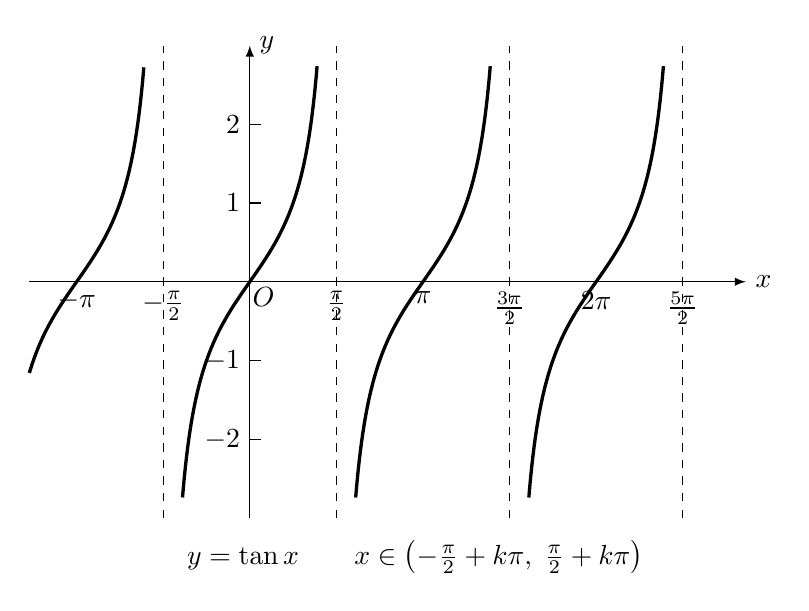
\begin{tikzpicture}[>=latex, xscale=.7]
    \draw[->] (-4,0)--(9,0)node[right]{$x$};
\draw[->] (0,-3)--(0,3)node[right]{$y$};
\foreach \x in {-.5,.5,1.5,2.5}
{
    \draw[dashed] (\x*pi,-3)--(\x*pi,3);
}

\foreach \y in {-.5,.5,1.5}
{
    \draw [domain=\y*pi+.35:(\y+1)*pi-.35, samples=1000, very thick] plot(\x, {tan(\x r)});
}

\draw [domain=-4:-.5*pi-.35, samples=1000, very thick] plot(\x, {tan(\x r)});

\foreach \z in {-2,-1,2,1}
{
    \draw (0,\z)node[left]{$\z$}--(.2,\z);
}

\node at (.25,-.2){$O$};
\node at (-pi,0)[below]{$-\pi$};
\node at (pi,0)[below]{$\pi$};
\node at (2*pi,0)[below]{$2\pi$};
\node at (-.5*pi,0)[below]{$-\frac{\pi}{2}$};
\node at (.5*pi,0)[below]{$\frac{\pi}{2}$};
\node at (1.5*pi,0)[below]{$\frac{3\pi}{2}$};
\node at (2.5*pi,0)[below]{$\frac{5\pi}{2}$};

\node at (3,-3.5){$y=\tan x\qquad x\in\left(-\frac{\pi}{2}+k\pi,\; \frac{\pi}{2}+k\pi\right)$};

\end{tikzpicture}
    \caption{}

\end{figure}

正切函数$y=\tan x$的图象叫做\textbf{正切曲线},由图7.9可以看出,正切曲线是由互相平行的直线$x=\frac{\pi}{2}+k\pi\;\;(k\in\mathbb{Z})$隔
开的无穷多支曲线所组成。

下面我们说明$y=\tan x$图象的几何画法。

应用单位圆上的正切线,我们在开区间$\left(-\frac{\pi}{2},\; \frac{\pi}{2}\right)$和$\left(\frac{\pi}{2},\; \frac{3\pi}{2}\right)$内作出正切函数$y=\tan x$的图象。画图象时
让横坐标每隔$\frac{\pi}{12}$
取点,作法如图7.10。

\begin{figure}[htp]
    \centering
    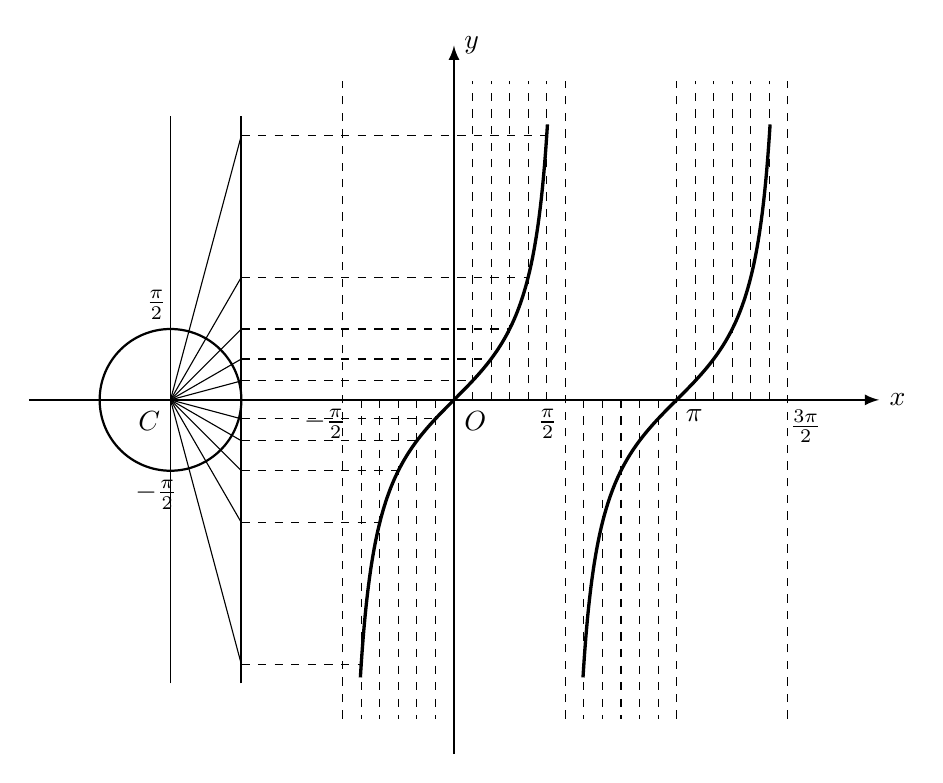
\begin{tikzpicture}[>=latex, scale=.9]
        \draw[->, thick] (-6,0)--(6,0)node[right]{$x$};   
\draw[->, thick] (0,-5)--(0,5)node[right]{$y$};
\draw[thick] (-4,0) circle(1);
\draw (-4,-4)--(-4,4);
\draw[thick] (-3,-4)--(-3,4);
\foreach \x in {-5,-4,...,5}
{
    \draw (-4,0) -- (-3, {tan(\x*pi/12 r)});
}

\foreach \y in {-.5,.5}
{
    \draw [domain=\y*pi+.25:(\y+1)*pi-.25, samples=1000, very thick] plot(\x, {tan(\x r)});
}

\foreach \x in {-5,-4,...,-1,7,8,...,11}
{
    \draw[dashed] (\x*pi/12,0)--(\x*pi/12,-4.5);
}
\foreach \x in {1,2,...,5,13,14,...,17}
{
    \draw[dashed] (\x*pi/12,0)--(\x*pi/12,4.5);
}
\foreach \x in {-1,1,2,3}
{
    \draw [dashed] (\x*pi/2, -4.5)--(\x*pi/2, 4.5);
}

\foreach \x in {-5,-4,...,5}
{
    \draw[dashed] (-3, {tan(\x*pi/12 r)})--(\x*pi/12, {tan(\x*pi/12 r)});
}
\node at (-4.3,-.3){$C$};
\node at (-4.2,1)[above]{$\frac{\pi}{2}$};
\node at (-4.2,-1)[below]{$-\frac{\pi}{2}$};
\node at (.3,-.3){$O$};
\node at (-pi/2-.25,0)[below]{$-\frac{\pi}{2}$};
\node at (pi/2-.25,0)[below]{$\frac{\pi}{2}$};
\node at (3*pi/2+.25,0)[below]{$\frac{3\pi}{2}$};
\node at (pi+.25,0)[below]{$\pi$};
    \end{tikzpicture}
    \caption{}
\end{figure}

\subsection{正切函数的主要性质}

由上一章的讨论和正切函数图象,我们可以得到正切函数$y=\tan x$的主要性质如下:

\begin{enumerate}
    \item 定义域\quad  正切函数$y=\tan x$的定义域是$x\ne \frac{\pi}{2}+k\pi, 
(k\in\mathbb{Z})$的一切实数,也就是由下面无数个开区间:
\[\left(-\frac{\pi}{2}+k\pi,\; \frac{\pi}{2}+k\pi\right),\quad k=0,\pm1,\pm2,\pm3,\ldots \]
组成的一个集。
\item 值域\quad  正切函数$y=\tan x$的值域为一切实数。
\item 奇偶性\quad 正切函数是奇函数。
\item 函数的符号\quad 当$x$在一、三象限时,$\tan x>0$; 在二、四象限时,$\tan x<0$. 一般地,
\begin{itemize}
    \item 若$x\in\left(2k\pi,\frac{\pi}{2}+2k\pi\right)$或$\left((2k+1)\pi,\frac{\pi}{2}+(2k+1)\pi\right)$时,$\tan x>0$;
    \item 若$x\in\left(\frac{\pi}{2}+2k\pi,(2k+1)\pi\right)$或$\left(\frac{\pi}{2}+(2k+1)\pi, 2k\pi\right)$时,$\tan x<0$。(这里$k\in\mathbb{Z}$)
\end{itemize}

 \item 增减性\quad 正切函数$y=tan x$在$x\in\left(-\frac{\pi}{2}+k\pi,\frac{\pi}{2}+k\pi\right)\;\; (k\in\mathbb{Z})$的每一个开区间内,都是递增的。

 但是要注意,正切函数在整个定义域内并不是增函数。事实上,设$x_1=\frac{\pi}{4}$, $x_2=\frac{3\pi}{4}$,那么
 \[\begin{split}
     \tan x_1&=\tan\frac{\pi}{4}=1\\
     \tan x_2&=\tan\frac{3\pi}{4}=\tan\left(\pi-\frac{\pi}{4}\right)=-\tan\frac{\pi}{4}=-1
 \end{split}\]
这样,$x_1<x_2$时,有$\tan x_1>\tan x_2$。
 当$x=k\pi$时 ($k\in\mathbb{Z}$), $\tan x=0$.
 
 \item 周期性\quad 由诱导公式$\tan (x+\pi)=\tan x$(这里$x$为定义域内任意数),知正切函数的周期是$\pi$, 现在我们证明$\pi$是正切函数的最小正周期。
 
\begin{proof}
    设$p$是$\tan x$的正周期且$0<p<\pi$,根据周期$p$的定义,我们有
$\tan (x+p)=\tan x$ (这里$x$是定义域内任意数)。

令$x=0$, 则$\tan p=\tan 0=0$, 由此得到$p=k\pi\;\; (k\in\mathbb{Z}, \text{且 }k\ne 0)$, 这就是说,如果$p$是$\tan x$的周期,$p$只能是$\pi$的整数倍,这就与存在比$\pi$小的正周期$p$的假设矛盾。

因此,$\pi$就是$\tan x$的最小正周期。
\end{proof}

\begin{itemize}
    \item 函数$y=\tan \omega x$的最小正周期是$\frac{\pi}{|\omega|}$ ($\omega\ne 0$,  $\omega x$为定义域内的数)。

    \item    函数$y=\tan (\omega x+\varphi)$的最小正周期是$\frac{\pi}{|\omega|}$ ($\omega,\varphi$为
    常数,且$\omega\ne 0$, $\omega x$为定义域内的数)。
\end{itemize}

\item  渐近线\quad 由图7.9可以看到,当$0<x<\frac{\pi}{2}$时,
$\tan x>0$, 又当$x<\frac{\pi}{2}$而$x$又无限地趋近$\frac{\pi}{2}$时,(记作$x\to \frac{\pi^-}{2}$),
正切曲线无限地下降但与直线$x=\frac{\pi}{2}$
永远不相交,我们把这个性质说成当$x$由小于$\frac{\pi}{2}$
的方面无限趋近$\frac{\pi}{2}$时,$\tan x$的值增大并超出任何指定的正数,并且写成
\[\lim_{x\to\tfrac{\pi^-}{2}}\tan x=+\infty  \]

当$\frac{\pi}{2}<x<\pi$时,$\tan x<0$,又当$x>\frac{\pi}{2}$,而且$x$无限地趋近$\frac{\pi}{2}$时(记作$x\to\frac{\pi^+}{2}$),
正切曲线无限地上升,但与直线$x=\frac{\pi}{2}$
永远不相交,我们把这个性质说成当$x$由大于$\frac{\pi}{2}$的方面无限趋近
$\frac{\pi}{2}$时,$\tan x$取负值减小但其绝对值增
大并超出任何指定的正数,并且写成
\[\lim_{x\to\tfrac{\pi^+}{2}}\tan x=-\infty  \]
同样地,还有
\[\lim_{x\to -\tfrac{\pi^-}{2}}\tan x=+\infty,\qquad  \lim_{x\to -\tfrac{\pi^+}{2}}\tan x=-\infty \]

我们把直线$x=-\frac{\pi}{2}$和$x=\frac{\pi}{2}$叫做正切曲线的渐近线。一般地,直线$x=(2k+1)\frac{\pi}{2},\;\; k\in\mathbb{Z}$都是正切曲线的渐近线。
\end{enumerate}

\begin{rmk}
    这里对渐近线的叙述,同学们只要从图象上了解其意义就可以了,这个问题到高中还要详细地介绍。 
\end{rmk}

\begin{ex}
\begin{enumerate}
    \item 证明$y=\tan\left(x-\frac{\pi}{2}\right)$是奇函数,作出它的图象。
    \item 作$y=-|\tan x|$的图象,并说出它的周期。
    \item 求下列函数的周期:
    \[\tan\left(2x-\frac{x}{4}\right),\qquad \tan \frac{x}{2} \]
\end{enumerate}
\end{ex}

\section{余切函数的图象和性质}
\subsection{余切函数的图象}

我们知道余切函数的定义域是除去$x=k\pi\;\; (k\in\mathbb{Z})$的实数集。也就是由下面无数个开区间$\ldots,(-2\pi ,-\pi ),\;(-\pi ,0),\;(0,\pi ),\;(\pi ,2\pi ),\ldots$ 组成的一个集,图象都在$k\pi\;\; (k\in\mathbb{Z})$处断开。

我们又知道余切函数是奇函数,故它的图象关于原点对称。

由关系式$\cot x=-\tan\left(x+\frac{\pi}{2}\right)$, 知道余切函数$\cot x$的
图象就是正切函数型$y=-\tan\left(x+\frac{\pi}{2}\right)$的图象,又$y=-\tan\left(x+\frac{\pi}{2}\right)$的图象
,可以通过将正切曲线$y=\tan x$沿$x$轴向左平移$\frac{\pi}{2}$个单位,再把所得曲线作关于$Ox$轴反射,这个最后得到的曲线就是余切函数$y=\cot x$的图象(如图7.11)。

\begin{figure}[htp]
    \centering
\begin{tikzpicture}[>=latex, scale=1]
\draw[->](-1,0)--(6,0)node[right]{$x$};
\draw[->](0,-4)--(0,4)node[right]{$y$};
\draw [domain=0+.3:pi-.3, thick, samples=1000] plot (\x, {tan(pi*.5 r+\x r)});
\draw [domain=0+.3:pi-.3, very thick, samples=1000] plot (\x, {-tan(\x r +pi*.5 r)});
\draw [domain=.5*pi+.3: 1.5*pi-.3, samples=1000] plot (\x, {tan(\x r)});

\foreach \x in {3,2,1,-1,-2,-3}
{
    \draw (0,\x)node[left]{$\x$}--(.1,\x);
}

\foreach \x/\xtext in {1/\tfrac{\pi}{2},2/\pi,3/\tfrac{3\pi}{2}}
{
    \draw [dashed] (\x*pi/2,-3.5)--(\x*pi/2,3.5);
    \node at (\x*pi/2+.2,0)[below]{$\xtext$};
}

\node at (-.2,-.2){$O$};
\foreach \x in {-1,-2,-3}
{
    \draw[dashed] (0,\x)--(pi,\x);
}
\foreach \x in {1,2,3}
{
    \draw[dashed] (0,\x)--(1.5*pi,\x);
}
\node at (3*pi/2-.35,3)[right]{$y=\tan x$};
\node at (2*pi/2,3.5){$y=\tan \left(x+\frac{\pi}{2}\right)$};
\node at (2*pi/2-.5,-3.5)[right]{$y=-\tan \left(x+\frac{\pi}{2}\right)=\cot x$};

\end{tikzpicture}
    \caption{}
\end{figure}


在具体画图时,我们也可以将正切函数$y=\tan x$的数值表作相应的改变得到余切函数$y=\cot x$的数值表,然后用描点法
作图.为此,只须将$\tan x$的自变数$x$的取值各减去$\frac{\pi}{2}$而使
原来的对应函数值都变为相应的相反数就可以了。今由正切函数$y=\tan x$, 在区间$\left(\frac{\pi}{2},\frac{3\pi}{2}\right)$上的数值表:

\begin{center}
\begin{tabular}{c|ccccccc}
\hline
$x$  &    $\frac{6\pi}{12}$  &    $\frac{7\pi}{12}$  &    $\frac{8\pi}{12}$  &    $\frac{9\pi}{12}$  &    $\frac{10\pi}{12}$  &    $\frac{11\pi}{12}$  \\    
\hline
$y=\tan x$   & 不存在  & $-3.73$  & $-1.73$  & $-1$  & $-0.58$  & $-0.27$  \\
\hline
$x$  &    $\pi$  &    $\frac{13\pi}{12}$  &    $\frac{14\pi}{12}$  &    $\frac{15\pi}{12}$  &    $\frac{16\pi}{12}$  &    $\frac{17\pi}{12}$ & $\frac{18\pi}{12}$ \\    
\hline
$y=\tan x$   & 0  & $0.27$  & $0.58$  & $1$  & $1.73$ & 3.73 & 不存在  \\
\hline
\end{tabular}    
\end{center}

作相应的改变后得到余切函数$y=\cot x$的数值表:
\begin{center}
\begin{tabular}{c|ccccccc}
\hline
$x$  &    $0$  &    $\frac{\pi}{12}$  &    $\frac{2\pi}{12}$  &    $\frac{3\pi}{12}$  &    $\frac{4\pi}{12}$  &    $\frac{5\pi}{12}$  \\    
\hline
$y=\cot x$   & 不存在  & $3.73$  & $1.73$  & $1$  & $0.58$  & $0.27$  \\
\hline
$x$  &    $\frac{6\pi}{12}=\frac{\pi}{2}$  &    $\frac{7\pi}{12}$  &    $\frac{8\pi}{12}$  &    $\frac{9\pi}{12}$  &    $\frac{10\pi}{12}$  &    $\frac{11\pi}{12}$ & $\frac{12\pi}{12}=\pi$ \\    
\hline
$y=\cot x$   & 0  & $-0.27$  & $-0.58$  & $-1$  & $-1.73$ & -3.73 & 不存在  \\
\hline
\end{tabular}    
\end{center}

根据此表,我们可以画出在区间$(0,\pi)$上的余切函数$y=\cot x$的图象。

余切函数$y=\cot x$的图象叫做\textbf{余切曲线}。整个余切曲线在点$x=k\pi\;\;(k\in\mathbb{Z})$处间断开,分成无数多个分支(图7.12)。

\begin{figure}[htp]
    \centering
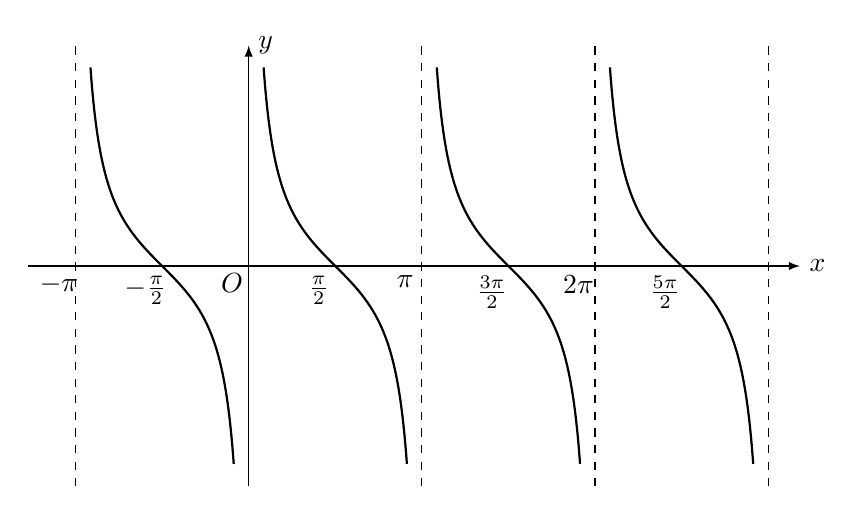
\begin{tikzpicture}[>=latex, scale=.7]
\draw[->] (-4,0)--(10,0)node[right]{$x$};
\draw[->] (0,-4)--(0,4)node[right]{$y$};
\foreach \x/\xtext in {-2/-\pi,-1/-\frac{\pi}{2},1/\frac{\pi}{2},2/\pi,3/\frac{3\pi}{2},4/2\pi,5/\frac{5\pi}{2}}
{
    \node at (\x*.5*pi-.3,0)[below]{$\xtext$};
}

\foreach \x in {-1,1,2,3}
{
    \draw[dashed] (\x*pi,-4)--(\x*pi,4);
}

\node at (-.3,-.3){$O$};

\foreach \y in {-1,1,3,5}
{
    \draw [domain=\y*0.5*pi-1.3 : \y*0.5*pi+1.3, samples=1000, thick] plot(\x, {cot (\x r) });
}

\end{tikzpicture}
    \caption{}
\end{figure}

\subsection{余切函数的主要性质}

由上一章的讨论和余切函数图象,我们可以得到余切函数$y=\cot x$的主要性质如下:
\begin{enumerate}
    \item 定义域\quad 余切函数$y=\cot x$的定义域是$x\ne k\pi\;\;(k\in\mathbb{Z})$的实数集,也就是由下面
无数个开区间:
\[\Bigl(k\pi,\; (k+1)\pi\Bigr), \qquad k=0,\pm1,\pm2,\pm3,\ldots\]
组成的一个集。

\item 值域\quad 余切函数$y=\cot x$的值域为一切实数。
\item 奇偶性\quad 余切函数是奇函数。
\item 函数的符号\quad 当$x$在第一、三象限时,$\cot x>0$;在第二、四象限时,$\cot x<0$,一般地:
\begin{itemize}
    \item 若$x\in\left(2k\pi,\;\frac{\pi}{2}+2k\pi\right)$或$\left((2k+1)\pi,\;\frac{\pi}{2}+(2k+1)\pi\right)$时,$\cot x>0$;
    \item 若$x\in\left(\frac{\pi}{2}+2k\pi,\; (2k+1)\pi\right)$或$\left(\frac{\pi}{2}+(2k+1)\pi,\; (2k+2)\pi\right)$时,$\cot x<0$,这里$k\in\mathbb{Z}$
\end{itemize}

\item 增减性\quad 余切函数$y=\cot x$在区间$(k\pi,\; (k+1)\pi)\;\; (k\in\mathbb{Z})$都是减函数。

当$x=\frac{\pi}{2}+2k\pi\;\; (k\in\mathbb{Z})$时,$\cot x=0$。

\item 周期性\quad 余切函数的周期是$\pi$。

事实上,假设$p>0$是$\cot x$的一个周期,根据周期$p$的定义,有$\cot (x+p)=\cot x$,这里x是$\cot x$的定义域中任何一个数。

令$x=\frac{\pi}{2}$,则
\[\cot\left(\frac{\pi}{2}+p\right)=\cot\frac{\pi}{2}\]
即$$\tan p=0$$
$\therefore\quad p=k\pi\quad (k\in\mathbb{Z},\; k\ne 0)$

由于$\cot(x+k\pi)=\cot x$对于$x$的任何容许值都成立,所以能使上面等式成立的最小正数$p=x$. 即$\cot x$的最小正周期等于$\pi$。

\begin{itemize}
    \item 函数$y=\cot \omega x$的最小正周期是$\frac{\pi}{|\omega|}$,($\omega\ne 0, \omega x$为定义域内的数)。
    \item 函数$y=A\cot (\omega x+\varphi)$的最小正周期是$\frac{\pi}{|\omega|}$,($\omega,\varphi$为常数,$\omega\ne 0, \omega x$为定义域内的数)。
\end{itemize}

\item 渐近线\quad 因为
\[\begin{split}
    \lim_{x\to 0^+} \cot x=+\infty,&\qquad \lim_{x\to 0^-} \cot x=-\infty\\
    \lim_{x\to \pi^-} \cot x=-\infty, &\qquad \lim_{x\to \pi^+} \cot x=+\infty
\end{split}\]
故$x=0$, $x=\pi$的直线就是余切曲线的渐近线。

一般地,直线$x=k\pi,\; (k\in\mathbb{Z})$,都是余切曲线的渐近线。

\end{enumerate}


\section*{习题7.3}
\addcontentsline{toc}{subsection}{习题7.3}

\begin{enumerate}
    \item 确定差的符号:
\begin{multicols}{2}
    \begin{enumerate}
\item $\tan 72^{\circ}-\tan 80^{\circ}$
\item $\cot 15^{\circ}-\cot 16^{\circ}$
\item $\tan 70^{\circ}-\cot 70^{\circ}$
\item $\cot 100^{\circ}-\cot 90^{\circ}$
    \end{enumerate}
\end{multicols}

\item 求下列各式子的符号:
\begin{multicols}{2}
    \begin{enumerate}
\item $\sin 3\cdot \tan 5$
\item $\cos 8\cdot \cos 5\cdot \tan 1$
\item $\tan 5\cdot \cot 3\cdot \tan 1$
\item $\sin(-5)\cos(-3)\tan(-2)\cot2$
    \end{enumerate}
\end{multicols}

\item 在怎样的区间内随着不超过$360^{\circ}$的正角$\alpha$的增大:
\begin{enumerate}
    \item $\sin\alpha$和$\cot\alpha$同时增大?同时减小?
    \item $\cos\alpha$和$\tan\alpha$同时增大?同时减小?
    \item $\sin\alpha$ 和 $\cos\alpha$同时增大?同时减小?
\end{enumerate}


\item 作下面函数的图象:
\[y=\cot\left(x-\frac{\pi}{2}\right),\qquad y=\cot\left(x+\frac{\pi}{3}\right) \]
\item 利用单位圆和余切函数线,解下面不等式
\[\cot x> 1,\qquad 3\cot x+\sqrt{3}<0\]

\item 作下面函数的图象:
\[y=\sec x,\qquad y=\csc x\]
\end{enumerate}


为了便于比较和查阅,我们把正弦函数,余弦函数,正切函数,余切函数的主要性质列表如下:

{\small
\begin{longtable}{p{.1\textwidth}|p{.18\textwidth}p{.18\textwidth}p{.18\textwidth}p{.18\textwidth}}
    \hline
函数 & $y=\sin x$ & $y=\cos x$    & $y=\tan x$ & $y=\cot x$\\
\hline
定义域 & $\mathbb{R}$ & $\mathbb{R}$ & $\{x|x\in \mathbb{R},\;\; x\ne\frac{\pi}{2}+k\pi\}$ & $\{x|x\in \mathbb{R},\;\; x\ne k\pi\}$\\
\hline
值域 & $[-1,1]$& $[-1,1]$& $\mathbb{R}$ &$\mathbb{R}$ \\
\hline
奇偶性 & 奇函数 &偶函数& 奇函数 &奇函数\\
\hline
函数的符号 & 在一、二象限为正;在三、四象限为负
& 在一、四象限为正;在二、三象限为负
& 在一、三象限为正;在二、四象限为负
& 在一、三象限为正;在二、四象限为负\\
\hline
增减性 & 在一、二象限是增函数;在三、四象限是减函数 
& 在一、二象限是减函数;在三、四象限是增函数 
& 在各象限都为增函数 
& 在各象限都为减函数 \\
\hline
函数的极值& $x=\frac{\pi}{2}+2k\pi$时,取极大值1;$x=\frac{3\pi}{2}+2k\pi$时,取极小值$-1$
& $x=2k\pi$时,取极大值1;$x=(2k+1)\pi$时,取极小值$-1$&无& 无\\
\hline
周期性& $2\pi$& $2\pi$& $\pi$& $\pi$\\
\hline
渐近线 & 无& 无& 直线$x=(2k+1)\frac{\pi}{2}$& 直线$x=k\pi$\\
\hline
\end{longtable}
}

\section{正弦型曲线}
在这一节,我们来研究正弦型曲线,即函数$y=A\sin(mx+a)$的图象,这个图象在学习物理、电工和力学时将会遇到,下面我们先研究几种特殊正弦型曲线的作法,然后再归结到一般情形。

\subsection{函数$y=A\sin x$ 的图象}

我们取$A=\frac{1}{2}$, $A=1$, $A=2$三种情形来讨论,即讨论
\[y=\frac{1}{2}\sin x,\qquad  y=\sin x,\qquad  y=2\sin x\]
考虑到函数$\sin x$的周期是$2\pi$, 我们只须画出闭区间$[0,
2\pi]$上的图象,先列出$x$由0到
$\frac{\pi}{2}$,每隔$\frac{\pi}{6}$取值的正弦
值表,然后,应用诱导公式$\sin(\pi-x)=\sin x$,
列出$\frac{\pi}{2}$
到$\pi$之间的正弦值;最后应用诱导公式
$\sin (\pi+x) =-\sin x$
列出$\pi$到$2\pi$之间的正弦值。
对于同一个$x$值,函数$\frac{1}{2}\sin x$的值为函数$\sin x$的值的$\frac{1}{2}$,而函数$2\sin x$的值为函数$\sin x$的值的2倍。

把它们的自变量及对应函数值列表于下:
\begin{center}
\begin{tabular}{cccc}
    \hline
$x$ & $y=\sin x$ & $y=\tfrac{1}{2}\sin x$ & $y=2\sin x$\\
\hline
$\cdots$ & $\cdots$&$\cdots$&$\cdots$\\
$0$   &    0   &   0 &  0\\
$\tfrac{\pi}{6}$   &    0.5   &   0.25 &  1\\
$\tfrac{\pi}{3}$   &    0.87   &   0.44 &  1.74\\
$\tfrac{\pi}{2}$   &    1   &   0.5 &  2\\
$\tfrac{2\pi}{3}$   &    0.87   &   0.44 &  1.74\\
$\tfrac{5\pi}{6}$   &    0.5   &   0.25 &  1\\
$\pi$   &    0   &   0 &  0\\
$\tfrac{7\pi}{6}$   &    $-0.5$   &   $-0.25$ &  $-1$\\
$\tfrac{4\pi}{3}$   &    $-0.87$   &   $-0.44$ &  $-1.74$\\
$\tfrac{3\pi}{2}$   &    $-1$   &   $-0.5$ &  $-2$\\
$\tfrac{5\pi}{3}$   &    $-0.87$   &   $-0.44$ &  $-1.74$\\
$\tfrac{11\pi}{6}$   &    $-0.5$   &   $-0.25$ &  $-1$\\
$2\pi$   &    0   &   0 &  0\\
$\cdots$ & $\cdots$&$\cdots$&$\cdots$\\
\hline
\end{tabular}
\end{center}

对于每一个函数,把表内$x$、$y$的每一对值作为点的坐标,在直角坐标系内作出对应点,将它们依次连结成平滑曲
线,这三条曲线就是正弦函数$y=\sin x$, 及正弦型函数$y=\frac{1}{2}\sin x$和$y=2\sin x$的图象(如图7.13).

\begin{figure}[htp]
    \centering
\begin{tikzpicture}[>=latex]
\draw [->](-1,0)--(7.8,0)node[right]{$x$};
\draw [->](0,-3)--(0,3)node[right]{$y$};
\foreach \x in {-1,-2,1,2}
{
    \draw(0,\x)node[left]{$\x$}--(.1,\x);
}

\node at (-.2,-.2){$O$};

\foreach \y in {1,2,.5}
{
    \draw [domain=0:7, samples=1000, thick] plot(\x, {\y*sin(\x r)});
}

\draw (.5*pi,0)node[below]{$\frac{\pi}{2}$}--(.5*pi,.1);

\draw (1.5*pi,0)--(1.5*pi,.1)node[above]{$\frac{3\pi}{2}$};

\node at (pi-.2,0)[below]{$\pi$};
\node at (2*pi+.2,0)[below]{$2\pi$};

\node at (7,.3)[right]{$y=\tfrac{1}{2}\sin x$};
\node at (7,.9)[right]{$y=\sin x$};
\node at (7,1.5)[right]{$y=2\sin x$};
\end{tikzpicture}
    \caption{}
\end{figure}


由图象显然看出:
\begin{enumerate}
    \item 对于同一横坐标$x$, $y=\frac{1}{2}\sin x$的纵坐标为$y=\sin x$的纵坐标的$\frac{1}{2}$,
    $y=2\sin x$的纵坐标为$y=\sin x$的纵坐标的2倍,
    因此,可以说,把曲线$y=\sin x$ 沿纵轴方向
    压缩到$\frac{1}{2}$,就得到曲线$y=\frac{1}{2}\sin x$; 沿纵轴方向拉长2
倍,就得到曲线$y=2\sin x$。

\item $y=\sin x$的最大纵坐标是1; $y=2\sin x$的最大纵坐标是2; $y=\frac{1}{2}\sin x$的最大纵坐标是$\frac{1}{2}$. 我们这个最大的纵坐标叫做该曲线的振幅。
\item 它们的周期相同,都是$2\pi$。
\end{enumerate}

推广到一般情形,就得出下面的结论:

\begin{blk}{}
    函数$y=A\sin x$的图象是把$y=\sin x$的图象沿着纵轴方向压缩到$A\; (0<A<1)$倍或拉长到$A\; (A>1)$倍而得到,曲线$y=A\sin x$的振幅为$A$, 周期为$2\pi$。
\end{blk}

\subsection{函数$y=\sin mx$的图象}

我们取$m=\frac{1}{2}$, $m=1$, $m=2$三种情形来讨论,即讨论$y=\sin\frac{x}{2}$, $y=\sin x$, $y=\sin2x$。

三个函数的周期分别是$4\pi$, $2\pi$和$\pi$, 它们有相同的振
幅$A=1$. 所有这些函数在自变量$mx$取相同值的变化过程中对应的函数值也相同,但现在$m$值不同,因此,只有当取不同的值时,才能使这些函数的对应值相同。
比如,
\begin{itemize}
    \item 当$x=\frac{\pi}{6}$时,$\sin x$的值为0.5;
    \item 当$x=\frac{\pi}{3}$时,$\sin \frac{1}{2}x$的值为0.5;
    \item 当$x=\frac{\pi}{12}$时,$\sin 2x$的值为0.5。
\end{itemize}

这就是说,只要我们有一个函数$y=\sin x$在闭区间$[0,2\pi]$上的函数值表,我们就可以通过把这个数值表中自变量
$x$的取值乘以2, 就得到函数$y=\sin\frac{1}{2}x$在闭区间$[0,4\pi]$上的函数值表;如果把$y=\sin x$的数值表中自变量$x$的取值除以2, 就可以得到$y=\sin 2x$在闭区间$[0,\pi]$上的函数值表。

列表作图于下:

将$y=\sin x$的函数值表
\begin{center}
\begin{tabular}{c|cccccccc}
\hline
$x$ &  $\cdots$   &  0    &  $\frac{\pi}{6}$     &   $\frac{\pi}{3}$     &   $\frac{\pi}{2}$      &  $\frac{2\pi}{3}$         &  $\frac{5\pi}{6}$ &  $\pi$  \\
\hline
$y=\sin x$ &  $\cdots$   &    0  & 0.5      &  0.87     &  1      &   0.87       &  0.5   & 0\\
\hline
$x$ &     & $\frac{7\pi}{6}$      &   $\frac{4\pi}{3}$     &  $\frac{3\pi}{2}$      &  $\frac{5\pi}{3}$       &    $\frac{11\pi}{6}$       &  $2\pi$ & $\cdots$   \\
\hline
$y=\sin x$ &      &  $-0.5$   &  $-0.87$    &   $-1$    & $-0.87$      &   $-0.5$     &   0      & $\cdots$\\
\hline
\end{tabular}
\end{center}
里的$x$的取值分别乘以2得到$y=\sin\frac{1}{2}x$的函数值表如下:
\begin{center}
\begin{tabular}{c|cccccccc}
\hline
$x$ &  $\cdots$   &  0    &  $\frac{\pi}{3}$     &   $\frac{2\pi}{3}$     &   $\pi$      &  $\frac{4\pi}{3}$         &  $\frac{5\pi}{3}$ &  $2\pi$  \\
\hline
$y=\sin\frac{1}{2}x$ &  $\cdots$   &    0  & 0.5      &  0.87     &  1      &   0.87       &  0.5   & 0\\
\hline
$x$ &     & $\frac{7\pi}{3}$      &   $\frac{8\pi}{3}$     &  $3\pi$      &  $\frac{10\pi}{3}$       &    $\frac{11\pi}{3}$       &  $4\pi$ & $\cdots$   \\
\hline
$y=\sin\frac{1}{2}x$ &      &  $-0.5$   &  $-0.87$    &   $-1$    & $-0.87$      &   $-0.5$     &   0      & $\cdots$\\
\hline
\end{tabular}
\end{center}

作图:
\begin{figure}[htp]
    \centering
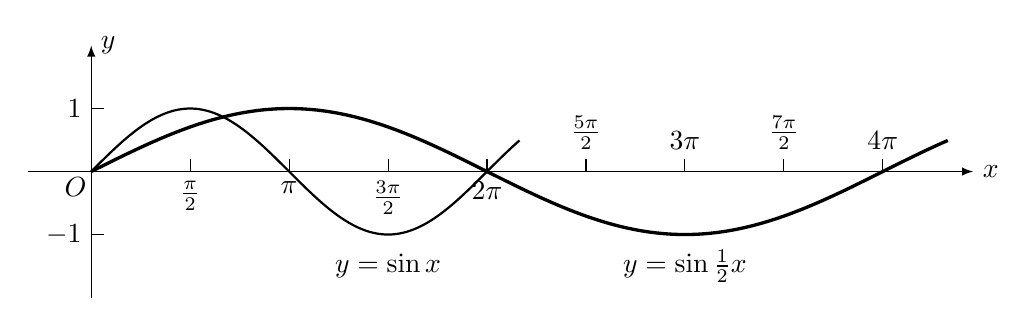
\begin{tikzpicture}[>=latex, scale=.8]
\draw[->] (-1,0)--(14,0)node[right]{$x$};
\draw[->]  (0,-2)--(0,2)node[right]{$y$};
\draw [domain=0:6.8, samples=1000, thick] plot(\x, {sin(\x r)});
\draw [domain=0:13.6, samples=1000, very thick] plot(\x, {sin(0.5*\x r)});
\node at (-.25,-.25){$O$};
\foreach \x in {-1,1}
{
    \draw (0,\x)node[left]{$\x$}--(.2,\x);
}
\foreach \x in {1,2,...,8}
{
    \draw (pi*\x/2,0)--(pi*\x/2,0.2);
}
\node at (pi/2,0)[below]{$\frac{\pi}{2}$};
\node at (pi,0)[below]{$\pi$};
\node at (3*pi/2,0)[below]{$\frac{3\pi}{2}$};
\node at (2*pi,0)[below]{$2\pi$};
\node at (5*pi/2,0.2)[above]{$\frac{5\pi}{2}$};
\node at (3*pi,0.2)[above]{$3\pi$};
\node at (7*pi/2,0.2)[above]{$\frac{7\pi}{2}$};
\node at (4*pi,0.2)[above]{$4\pi$};
\node at (3*pi/2,-1.5){$y=\sin x$};
\node at (3*pi,-1.5){$y=\sin \frac{1}{2}x$};
\end{tikzpicture}
    \caption{}
\end{figure}

由上面的表和图7.14可以看出:
\begin{enumerate}
    \item 当$y=\sin\frac{1}{2}x$的横坐标为$y=\sin x$的横坐标的2倍时,它们的纵坐标相等。
    \item 它们的振幅相同,都是1.
    \item $y=\sin\frac{1}{2}x$的周期是$4\pi=\frac{2\pi}{1/2}$,
二倍于$y=\sin x$的周期。
\end{enumerate}

因此,$y=\sin\frac{1}{2}x$的图象是把$y=\sin x$的图象沿横轴方向拉长2倍而得到。

将$y=\sin x$的函数值表里的$x$取值分别除以2, 得到$y=\sin 2x$的函数值如下:
\begin{center}
\begin{tabular}{c|cccccccc}
\hline
$x$ &  $\cdots$   &  0    &  $\frac{\pi}{12}$     &   $\frac{\pi}{6}$     &   $\frac{\pi}{4}$      &  $\frac{\pi}{3}$         &  $\frac{5\pi}{12}$ &  $\frac{\pi}{2}$  \\
\hline
$y=\sin\frac{1}{2}x$ &  $\cdots$   &    0  & 0.5      &  0.87     &  1      &   0.87       &  0.5   & 0\\
\hline
$x$ &     & $\frac{7\pi}{12}$      &   $\frac{2\pi}{3}$     &  $\frac{3\pi}{4}$      &  $\frac{5\pi}{6}$       &    $\frac{11\pi}{12}$       &  $\pi$ & $\cdots$   \\
\hline
$y=\sin\frac{1}{2}x$ &      &  $-0.5$   &  $-0.87$    &   $-1$    & $-0.87$      &   $-0.5$     &   0      & $\cdots$\\
\hline
\end{tabular}
\end{center}

作图象:
\begin{figure}[htp]
    \centering
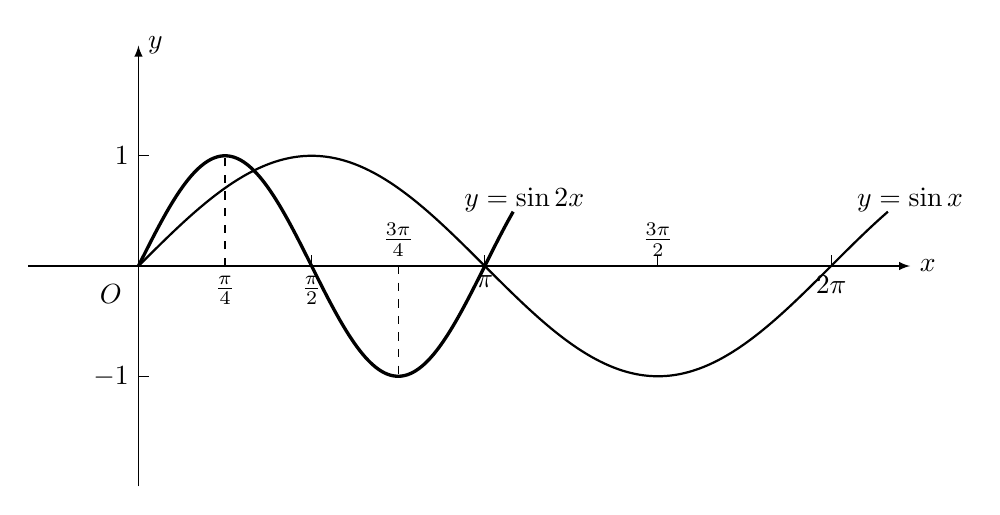
\begin{tikzpicture}[>=latex, scale=1.4]
\draw[->] (-1,0)--(7,0)node[right]{$x$};
\draw[->]  (0,-2)--(0,2)node[right]{$y$};
\draw [domain=0:6.8, samples=1000, thick] plot(\x, {sin(\x r)});
\draw [domain=0:3.4, samples=1000, very thick] plot(\x, {sin(2*\x r)});
\node at (-.25,-.25){$O$};
\foreach \x in {-1,1}
{
    \draw (0,\x)node[left]{$\x$}--(.1,\x);
}
\foreach \x in {1,2,3,4}
{
    \draw (pi*\x/2,0)--(pi*\x/2,0.1);
}
\node at (pi/2,0)[below]{$\frac{\pi}{2}$};
\node at (pi,0)[below]{$\pi$};
\node at (3*pi/2,0)[above]{$\frac{3\pi}{2}$};
\node at (2*pi,0)[below]{$2\pi$};
\node at (pi/4,0)[below]{$\frac{\pi}{4}$};
\node at (pi/4*3,0)[above]{$\frac{3\pi}{4}$};
\draw[dashed] (pi/4,0)--(pi/4,1);
\draw[dashed] (pi/4*3,0)--(pi/4*3,-1);
\node at (7,.6){$y=\sin x$};
\node at (3.5,.6){$y=\sin 2x$};


\end{tikzpicture}
    \caption{}
\end{figure}

由上面的表和图7.15可以看出:
\begin{enumerate}
    \item 当$y=\sin2x$的横坐标为$y=\sin x$的横坐标的一半时,它们的纵坐标相等。
    \item 它们的振幅相同,都是1.
    \item $y=\sin2x$的周期是$\pi\left(=\frac{\pi}{2}\right)$
\end{enumerate}

因此,$y=\sin2x$的图象是把曲线$y=\sin x$沿横轴方向压缩$\frac{1}{2}$倍,就得到曲线$y=\sin2x$.

根据上述情况,可得一般结论如下:

\begin{blk}{}
   函数$y=\sin mx$的图象是把$y=\sin x$的图象沿横轴方向拉长$\frac{1}{m}$倍$(0<m<1)$,或压缩到$\frac{1}{m},\; (m>1)$而得到。曲线$y=\sin mx$的振幅为1, 周期为$\frac{2\pi}{m}$。 
\end{blk}

\subsection{函数$y=A\sin(mx+\alpha)$的图象}

现在我们来说明如何画一般的正弦型曲线$y=A\sin(mx+\alpha)$. 这里$A$和$m$为已给的正实数,$\alpha$为已给的实数。

把函数
\begin{equation}
    y=A\sin(mx+\alpha)
\end{equation}
改写成
\begin{equation}
    y=A\sin m\left(x+\frac{\alpha}{m}\right)
\end{equation}
函数(7.5), (7.6)和函数$y=A\sin mx$的振幅相同,都等于$A$. 而且它们的周期也相同,都等于$\frac{2\pi}{m}$.

显然,$y=A\sin m\left(x+\frac{\alpha}{m}\right)$的图象上一点的横坐标$x_1$所对应的纵坐标是$y=A\sin m\left(x_1+\frac{\alpha}{m}\right)$, 并且恒等于$y=A\sin mx$的图象上横坐标是
$x_1+\frac{\alpha}{m}$的一点的纵坐标。由于在$Ox$轴上点$x_1$是在点$x_1+\frac{\alpha}{m},\;(\alpha>0)$的左方$\left|\frac{\alpha}{m}\right|$个单位处,或者点$x_1$是在点$x_1+\frac{\alpha}{m},\;(\alpha<0)$的右方的$\left|\frac{\alpha}{m}\right|$个单位处,所以我们只须把
$y=A\sin mx$的图象沿横轴方向左移$x_1+\frac{\alpha}{m},\;(\alpha>0)$个单位,或者右移$x_1+\frac{\alpha}{m},\;(\alpha<0)$个单位,就得到$y=A\sin m\left(x+\frac{\alpha}{m}\right)$的图象。

\begin{example}
作函数$y=1.5\sin \left(2t+\frac{\pi}{4}\right)$的图象。
\end{example}

\begin{solution}
所求函数$y=1.5\sin \left(2t+\frac{\pi}{4}\right)$的图象,可以由函数$y=1.5\sin 2t$的图象沿横轴方向左移$\frac{\pi}{8}$个单位得到。这时,曲线$y=1.5\sin2t$上的$(0, 0)$点就平移到$\left(-\frac{\pi}{8},0\right)$
点,我们把它作为曲线$y=1.5\sin2 \left(t+\frac{\pi}{8}\right)$的起点。

列出函数$y=\sin t$在闭区间$[0, 2\pi]$上自变量$t$每隔$\frac{\pi}{4}$的函数值表:
\begin{center}
\begin{tabular}{c|ccccccccc}
    \hline
$t$  &  0  &  $\frac{\pi}{4}$ & $\frac{\pi}{2}$   & $\frac{3\pi}{4}$  & $\pi$   & $\frac{5\pi}{4}$  & $\frac{3\pi}{2}$   & $\frac{7\pi}{4}$ &$2\pi$ \\ 
    \hline
$y=\sin t$  & 0   &   0.71 &  1 & 0.71   & 0  & $-$0.71   &  $-$1 & $-$0.71   & 0\\
    \hline
\end{tabular}
\end{center}

按照给出的曲线方程作相应的变更,分别得到函数$y=\sin2t$, $y=1.5\sin2t$和$y=1.5\sin2\left(t+\frac{\pi}{8}\right)$在一个周期内的函数值表如下:
\begin{center}
\begin{tabular}{c|ccccccccc}
    \hline
$t$  &  0  &  $\frac{\pi}{8}$ & $\frac{\pi}{4}$   & $\frac{3\pi}{8}$  & $\frac{\pi}{2}$   & $\frac{5\pi}{8}$  & $\frac{3\pi}{4}$   & $\frac{7\pi}{8}$ &$\pi$ \\ 
    \hline
$y=\sin 2t$  & 0   &   0.71 &  1 & 0.71   & 0  & $-$0.71   &  $-$1 & $-$0.71   & 0\\
$y=1.5\sin 2t$ & 0   &   1.07 &  1.5 & 1.07   & 0  & $-$1.07   &  $-$1.5 & $-$1.07   & 0\\
    \hline
\end{tabular}
\end{center}

\begin{center}
\begin{tabular}{c|ccccc}
    \hline
$t$  &  $-\frac{\pi}{8}$ & 0 & $\frac{\pi}{8}$   & $\frac{\pi}{4}$  & $\frac{3\pi}{8}$   \\     \hline
$y=1.5\sin \left(2t+\frac{\pi}{4}\right)$  & 0   &   1.07 &  1.5 & 1.07   & 0 \\
    \hline
    $t$  && $\frac{\pi}{2}$  & $\frac{5\pi}{8}$   & $\frac{3\pi}{4}$ &$\frac{7\pi}{8}$ \\
    \hline
    $y=1.5\sin \left(2t+\frac{\pi}{4}\right)$  &  & $-$1.07   &  $-$1.5 & $-$1.07   & 0\\
    \hline
\end{tabular}
\end{center}

作图:
\begin{figure}[htp]
    \centering
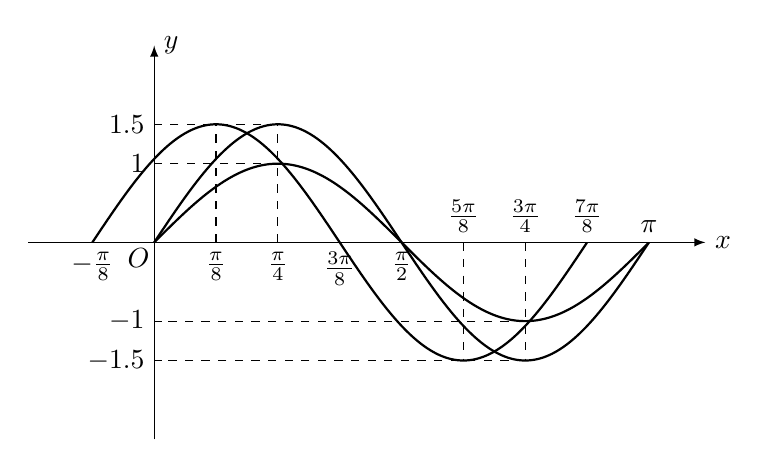
\begin{tikzpicture}[>=latex, xscale=2]
\draw[->](-.8,0)--(3.5,0)node[right]{$x$};
\draw[->] (0,-2.5)--(0,2.5)node[right]{$y$};    

\draw [domain=0:pi, samples=1000, thick] plot(\x, {sin(2*\x  r)});
\draw [domain=0:pi, samples=1000, thick] plot(\x, {1.5*sin(2*\x  r)});
\draw [domain=-pi/8:pi*7/8, samples=1000, thick] plot(\x, {1.5*sin(2*\x r +pi/4  r)});
\node at (-.1,-.2){$O$};

\foreach \x/\xtext in {-1/-\frac{\pi}{8},1/\frac{\pi}{8},2/\frac{\pi}{4},3/\frac{3\pi}{8},4/\frac{\pi}{2}}
{
    \node at (\x*pi/8,0)[below]{$\xtext$};
}

\foreach \x/\xtext in {5/\frac{5\pi}{8},6/\frac{3\pi}{4},7/\frac{7\pi}{8},8/\pi}
{
    \node at (\x*pi/8,0)[above]{$\xtext$};
}

\foreach \x in {1,2}
{
    \draw[dashed] (\x*pi/8,0)--(\x*pi/8,1.5);
    \draw[dashed] (\x*pi/8+0.5*pi,0)--(\x*pi/8+0.5*pi,-1.5);
}

\draw[dashed](pi/4,1.5)--(0,1.5);  \draw[dashed](pi/4,1)--(0,1);
\draw[dashed](3*pi/4,-1.5)--(0,-1.5);  \draw[dashed](3*pi/4,-1)--(0,-1);

\foreach \x in {-1.5,-1,1,1.5}
{
    \draw (0,\x)node[left]{$\x$}--(.05,\x);
}
\end{tikzpicture}
    \caption{}
\end{figure}
\end{solution}

上面这种作图方法,把几种曲线之间的关系明确的揭露出来,使我们能够了解到它们之间的内在联系,但是,这样作图比较费事,在实际问题中往往只须知道函数
$y=A\sin(mx+\alpha)$的草图,只要这个图能够表示出它的
三个特征量:
振幅$A$, 周期$\frac{2\pi}{m}$,起点$\left(-\frac{\alpha}{m},0\right)$就可以了。

$y=A\sin(mx+\alpha)$的图象的简便作法如下:
\begin{enumerate}
    \item 化函数$y=A\sin(mx+\alpha)$为下面的形式
    \[y=A\sin m\left(x+\frac{\alpha}{m}\right)\]
    \item 确定:振幅为$A$; 周期为$\frac{2\pi}{m}$;起点为$\left(-\frac{\alpha}{m},0\right)$。
    \item 选取比例尺:1个单位为几厘米。
    \item 在$Ox$轴上以$\left(-\frac{\alpha}{m},0\right)$为起点,并把$x=-\frac{\alpha}{m}$
到$x=-\frac{\alpha}{m}+\frac{2\pi}{m}$的一段分成4等份,每等份长为$\frac{2\pi}{m}\div 4=\frac{\pi}{2m}$, 各分点的横坐标是
\[-\frac{\alpha}{m},\quad  -\frac{\alpha}{m}+\frac{\pi}{2m},\quad -\frac{\alpha}{m}+\frac{\pi}{m},\quad -\frac{\alpha}{m}+\frac{3\pi}{2m},\quad -\frac{\alpha}{m}+\frac{2\pi}{m}  \]
它们对应的纵坐标分别是$0, A,0,-A,0$。
\end{enumerate}

根据上述结果,便可作出函数$y=A\sin (mx+\alpha)$在区间$\left[-\frac{\alpha}{m},\; -\frac{\alpha}{m}+\frac{2\pi}{m}\right]$上的图象。


\begin{example}
求作函数$y=\frac{3}{2}\sin(3t-\pi)$的图象。
\end{example}

\begin{solution}
\begin{enumerate}
    \item 化函数$y=\frac{3}{2}\sin(3t-\pi)$为下面的形式:
    \[y=\frac{3}{2}\sin 3\left(t-\frac{\pi}{3}\right)\]
\item 确定:振幅为$\frac{3}{2}$,周期为$\frac{2\pi}{8}$,起点为$\left(\frac{\pi}{8},\; 0\right)$
\item 选取比例尺:1个单位长$=0.8$厘米。
\item 列表:
\begin{center}
    \begin{tabular}{c|ccccccc}
  \hline      
$t$   &  $\cdots$  & $\frac{\pi}{3}$  & $\frac{\pi}{2}$  & $\frac{2\pi}{3}$  & $\frac{5\pi}{6}$  & $\pi$ &$\cdots$\\
\hline
$y=\frac{3}{2}\sin(3t-\pi)$ &  $\cdots$  & 0 & $\frac{3}{2}$ &0 &$-\frac{3}{2}$ & 0&$\cdots$\\
\hline
    \end{tabular}
\end{center}
  \end{enumerate}  


\begin{figure}[htp]
    \centering
\begin{tikzpicture}[scale=1.3, >=latex]
\draw[->] (-2,0)--(7,0)node[right]{$x$};
\draw[->] (0,-2.5)--(0,2.5)node[right]{$y$};
\draw [domain=-pi/3:2*pi, samples=1000, dashed] plot(\x, {1.5*sin(3*\x r - pi r)});
\draw [domain=pi/3:pi, samples=1000, very thick] plot(\x, {1.5*sin(3*\x r - pi r)});
\node at (-.2,-.2){$O$};

\foreach \x/\xtext in {-2/-\frac{\pi}{3},-1/-\frac{\pi}{6},1/\frac{\pi}{6},3/\frac{\pi}{2},5/\frac{5\pi}{6},7/\frac{7\pi}{6},9/\frac{3\pi}{2},11/\frac{11\pi}{6}}
{
    \draw (\x*pi/6,0)node[below]{$\xtext$}--(\x*pi/6,.1);
}

\foreach \x/\xtext in {2/\frac{\pi}{3},4/\frac{2\pi}{3},6/\pi,8/\frac{4\pi}{3},10/\frac{5\pi}{3},12/2\pi}
{
    \draw (\x*pi/6,0)--(\x*pi/6,.1)node[above]{$\xtext$};
}

\foreach \x in {-1.5,-1,1,1.5}
{
    \draw(0,\x)node[left]{$\x$}--(.1,\x);
}


\end{tikzpicture}
    \caption{}
\end{figure}
\end{solution}


图中虚线表示曲线$y=\frac{3}{2}\sin(3t-\pi)$上未画出的部分,我们把图象变换总结如下:

\begin{blk}{位置变换}
\begin{enumerate}
    \item $y=\sin(x+b)$的图象可由$y=\sin x$的图象沿$x$轴的方向左、右平移而得到(当$b>0$时向左,$b<0$时向右)。
    \item $y=\sin x+\ell$的图象可由$y=\sin x$的图象沿$y$轴的方向上、下平移而得到(当$\ell>0$时向上,$\ell<0$时向下)。
    \item $y=-\sin x$的图象可由$y=\sin x$的图象作关于$Ox$轴的反射得到。
\end{enumerate}
\end{blk}

\begin{blk}{形状变换}
    \begin{enumerate}
        \item $y=A\sin x\; (A>0)$的图象可由$y=\sin x$的图象的振幅扩大$A$倍而得到。
\item $y=\sin mx\; (m>0)$的图象可由$y=\sin x$的图象沿$x$轴方向拉长($0<m<1$)或压缩($m>1$)到$\frac{1}{m}$倍而得到(周期$T$为$\frac{2\pi}{m}$)。
    \end{enumerate}
\end{blk}


\begin{blk}{位置形状全变换}
\[y=A\sin(mx+\alpha)+\ell=A\sin m\left(x+\frac{\alpha}{m}\right) +\ell\quad  (A> 0,\; m>0)\]
可由$y=\sin x$的图象沿轴方向拉长或压缩到原来的
$\frac{1}{m}$倍,(周期变为$\frac{2\pi}{m}$), 沿$x$轴向左或向右平移$\left|\frac{\alpha}{m}\right|$
个单位,然后把振幅扩大到原来的$A$倍;最后沿$y$轴向上或向下平移$|\ell|$个单位。
\end{blk}

\begin{ex}
\begin{enumerate}
    \item 作下面三角函数的图象:
    \begin{multicols}{2}
\begin{enumerate}
    \item $y=1+\sin2x$
    \item $y=\sin\left(x+\frac{\pi}{4}\right) $
    \item $y=2\sin\left(3t-\frac{\pi}{3}\right)$
    \item $y=\frac{2}{3}\cos\left(\frac{1}{2}x+\frac{\pi}{4}\right)$
\end{enumerate}
    \end{multicols}
    \item 求下面函数的图象在$(0, 2\pi)$区间的交点坐标:
    \begin{enumerate}
        \item $y=\sin 2x$和$y=2\cos x$
        \item $y=\sin 3x$和$y=2\sin x$
    \end{enumerate}
\end{enumerate}
\end{ex}

\section*{复习题七}
\addcontentsline{toc}{section}{复习题七}
\begin{enumerate}
    \item 求$\theta$所在的象限,已知:
\begin{multicols}{2}
\begin{enumerate}
    \item $\sin\theta$和$\cot \theta$同号
    \item $\cos\theta$和$\tan \theta$异号
    \item $\frac{\tan\theta}{\cot\theta}$是正值
    \item $\sin\theta <0$,而$\cos\theta>0$
\end{enumerate}
\end{multicols}
\item 根据三角函数性质,比较两函数值的大小:
\begin{multicols}{2}
    \begin{enumerate}
        \item $\sin 20^{\circ},\qquad \sin 21^{\circ}$
        \item $\cos 20^{\circ},\qquad \cos 120^{\circ}$
        \item $\tan 120^{\circ},\qquad \tan 121^{\circ}$
        \item $\cot175^{\circ},\qquad \cot 185^{\circ}$
        \item $\cos 1^{\circ},\qquad \cos 1$
        \item $\sin 1,\qquad \cos 1$
        \item $\sin(-310^{\circ}),\qquad \cos(-310^{\circ})$
        \item $\sin\frac{4\pi}{5},\qquad \cos\frac{4\pi}{5}$
    \end{enumerate}
    \end{multicols}


\item 说出下列各函数的周期:
\begin{multicols}{2}
\begin{enumerate}
    \item $y=\sin 4x$
    \item $y=\cos\frac{x}{2}$
    \item $y=\tan ax \quad (a>0)$
    \item $y=\sin\left(x+\frac{\pi}{8}\right)$
    \item $y=\cos\left(2x-\frac{\pi}{6}\right)$
    \item $y=3\tan\left(\frac{x}{2}+\frac{\pi}{4}\right)$
\end{enumerate}
\end{multicols}

\item \begin{enumerate}
    \item 等式$\sin\left(\frac{7\pi}{6}+\frac{2\pi}{3}\right)=\sin\frac{7\pi}{6}$,能不能成立?
    \item 如果上面的等式成立,能不能说$\frac{2\pi}{3}$是$\sin x$的周期?为什么?
\end{enumerate}

\item \begin{enumerate}
    \item 等式$\sin(x+4\pi)=\sin x$是不是对于$x$的一切值都能成立?
    \item 如果上面的等式对于$x$的一切值都能成立,能不能说$4\pi$是$\sin x$的周期?为什么?
\end{enumerate}

\item 用下面给出的周期,各举出一个周期函数来:
\[3\pi,\qquad \frac{\pi}{6},\qquad \frac{2\pi}{3}\]

\item 说明正弦曲线$y=\sin x$经过怎样的变化能得到下列的
函数曲线:
\begin{multicols}{2}
\begin{enumerate}
    \item $y=\frac{1}{2}\sin 3x$
    \item $y=2\sin\left(x+\frac{\pi}{4}\right)$
    \item $y=\sin\left(2x+\frac{\pi}{2}\right)$
    \item $y=2\sin\left(3x-\frac{\pi}{8}\right)$
\end{enumerate}
\end{multicols}

\item 电流强度$I$随时间$t$变化的函数关系是$I=A\sin\omega t$。设$\omega=100\pi$(弧度/秒),$A=5$(安培):
\begin{enumerate}
    \item 求电流强度变化的周期和频率(往复振动一次所需
的时间$T=\frac{2\pi}{\omega}$, 叫做振动的周期,单位时间内往复振动的
次数$f=\frac{1}{T}=\frac{\omega}{2\pi}$,叫做振动的频率);
\item 当$t=0$、$\frac{1}{200}$、$\frac{1}{100}$、$\frac{3}{200}$、$\frac{1}{50}$(秒)时,求电流强度;
\item 画出图象表示电流强度$I$随时间$t$的变化情况(以
$I$为纵坐标,0.5cm表示1安培;以$t$为横坐标,1cm表示$\frac{1}{200}$秒)。
\end{enumerate}

\item 如图,一质点$P$在线段$CC'$上作往复运动,取原点
$O$为$CC'$中点,又$CC'=16$cm, 设$P$点离开原点$O$的坐
标$x$是时间$t$的函数$x=8\sin\left(\frac{\pi}{4}t+\frac{\pi}{6}\right)$
\begin{center}
    \begin{tikzpicture}
   \draw (-5,0)--(5,0);
\foreach \x/\xtext in {-4/C,0/O,4/C'}
{
    \draw (\x,0) [fill=black] circle(1.5pt)node[below]{$\xtext$};
}        

\draw (1,0) [fill=black] circle(1.5pt)node[above]{$P$};
    \end{tikzpicture}
\end{center}
问: \begin{enumerate}
\item 当$t=0, 2, 4$秒时,$P$点在何位置?
\item 从0秒算起,经过多少秒,$P$点第一次到达$C$点。
\item 经过多少秒后$P$点开始重复运动。
\end{enumerate}


\end{enumerate}
